 \documentclass[11pt,conference,compsoc]{IEEEtran}

\usepackage{lipsum} 
% *** CITATION PACKAGES ***
%
\ifCLASSOPTIONcompsoc
  \usepackage[nocompress]{cite}
\else
  \usepackage{cite}
\fi

\usepackage{microtype}
\usepackage{booktabs} 

\usepackage{graphicx} 
\usepackage{subcaption}

\usepackage{booktabs,subcaption,amsfonts,dcolumn}
\newcolumntype{d}[1]{D..{#1}}
\newcommand\mc[1]{\multicolumn{1}{c}{#1}} 

\usepackage[usenames, dvipsnames]{color}
\newcommand{\ts}{\textsuperscript}

\usepackage{graphicx}
\ifCLASSINFOpdf

\hyphenation{op-tical net-works semi-conduc-tor}

\usepackage{tabularx}

\begin{document}

\title{Artificial Neural Networks and Deep Learning}

\author{\IEEEauthorblockN{Angelos Evmorfopoulos}
\IEEEauthorblockA{Master of Engineering: Computer Science, Artificial Intelligence\\
KU Leuven\\
2019-2020\\
}}
% make the title area
\maketitle

\thispagestyle{plain}
\pagestyle{plain}


\section{Supervised learning and generalization}

\subsection{Backpropagation in Feedforward Multi-Layer Networks}

\subsubsection{Function Approximation and Learning from Noisy Data\\}

The aim of this exercise is to approximate the function $y=sin(x^2)$ by using a feedforward neural network with one hidden layer. In general, function approximation is a technique for approximating or estimating a previously unknown underlying function by using observations from the domain. The reason for using a single hidden layer is expressed in the universal approximation theorem in mathematics for artificial neural networks, which states that the first layer, in our case the single hidden layer, can approximate any desired function, therefore there is no need for any additional layers. 

In order to approximate the aforementioned function, the following training algorithms were used: gradient descent (\textit{traingd}), gradient descent with adaptive learning rate (\textit{traingda}), Fletcher-Reeves conjugate gradient (\textit{traincfg}), Polak-Ribiere conjugate gradient (\textit{traincgp}), BFGS quasi Newton (\textit{trainbfg}), Levenberg-Marquardt (\textit{trainlm}) and, finally, Levenberg-Marquardt with Bayesian regularization (\textit{trainbr}). The first part of the experiment is to evaluate and compare their performance based on their training parameters, namely the amount of training examples, the amount of neurons in the hidden layer and the number of epochs in training. The second part of the experiment is to evaluate once again their performance but instead of having noiseless data we add noise and then compare the results in contrast to the noiseless data. The performance metrics utilized are the average R values and training times of these algorithms over ten runs, which are then aggregated and visualised in Figure 1.

\textbf{Number of Hidden Neurons:} The amount of hidden neurons in the network varied, starting from 5 to 10, 20, 50 and 100. Increasing the number of neurons to 300 was also attempted but training time drastically increased, since by doing so the model became more complex and therefore requires more time. An interesting observation is that for the majority of the training algorithms, 50 neurons are sufficient to produce a good result, whereas numbers higher than 50 increase variance and had worse results. Finally, by using a lower number of neurons leads to higher bias and, in general, results in a less expressive model that is prone to underfitting.

\textbf{Number of Training Examples:} The initial amount of training samples was 189, then increased to 315 and, finally, to 943. Understandably, as the amount of samples increases, the performance of the algorithms also improves, since more information is provided to the neural network in order to solve the task at hand.

\textbf{Number of Epochs:} The number of epochs was varied from 10 to 50, 100, 200 and 1000. Understandably, as the number of epochs increases, the performance also improves, considering that every time the training algorithms are able to explore a larger part of the search space. However, very high numbers of epochs may lead to overfitting. 

\textbf{Introduction of noise to data:} In this part of the exercise we introduce noise to the data, which varies from 0 to 0.4. As we can observe in Figure 2, the introduction of noise lowers the R values of the training algorithms. The algorithm that performs better after the addition of noise is Levenberg-Marquardt (\textit{trainlm}). 

\begin{figure*}[]

    \begin{subfigure}{0.33\linewidth}
        %\centering
        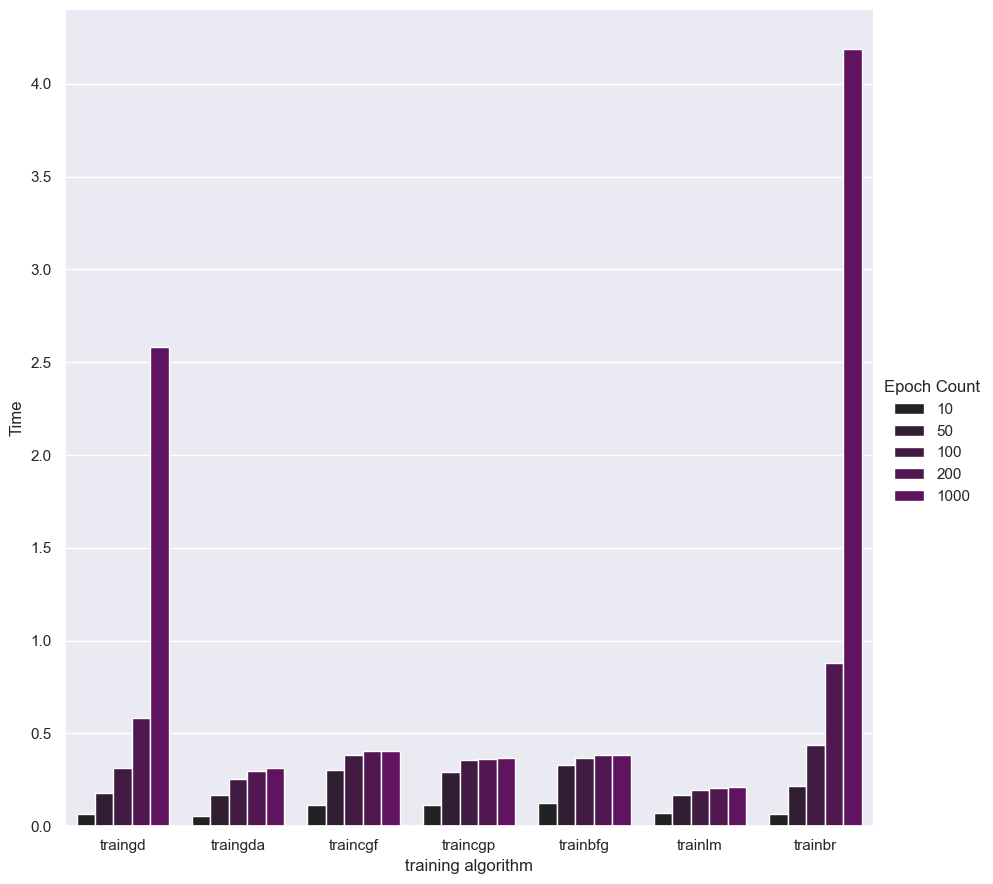
\includegraphics[width=\linewidth]{images/Epochs-Time.png}
        \caption{Number of Epochs - Time}
    \end{subfigure}
    \begin{subfigure}{0.33\linewidth}
        %\centering
        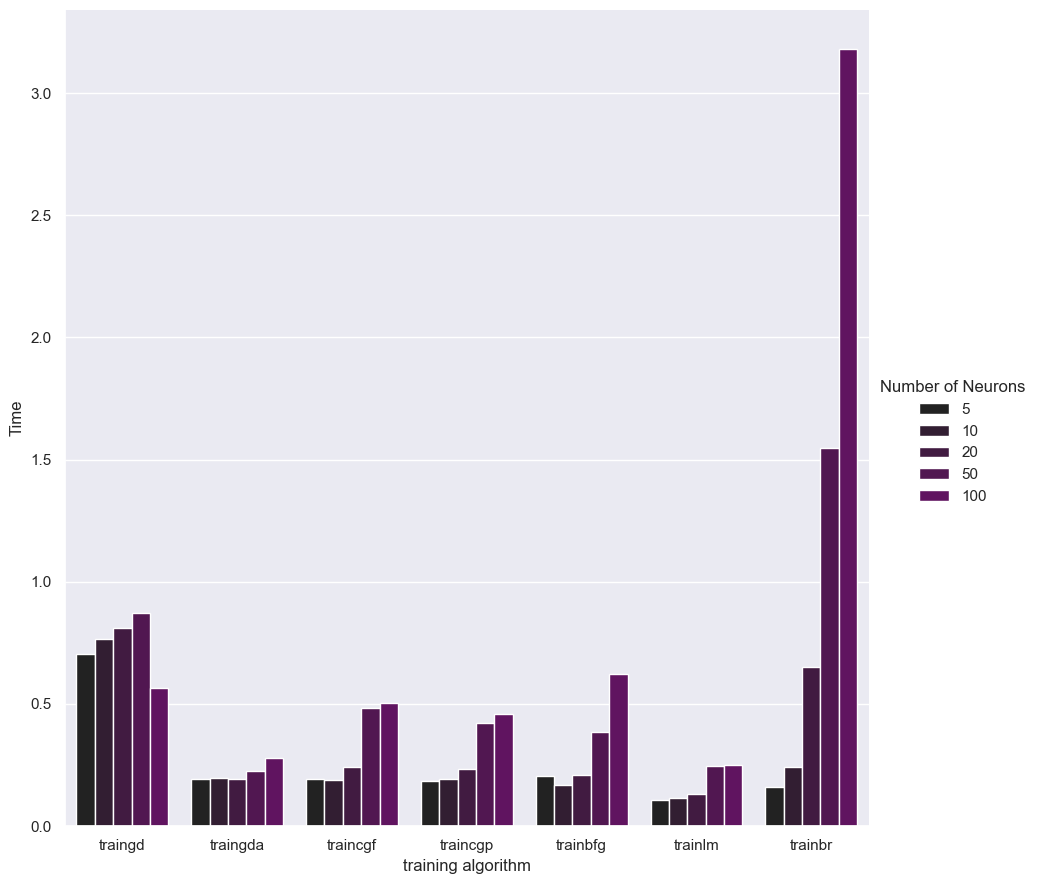
\includegraphics[width=\linewidth]{images/Neurons-Time.png}
        \caption{Number of Neurons - Time}
    \end{subfigure}
    \begin{subfigure}{0.33\linewidth}
        %\centering
        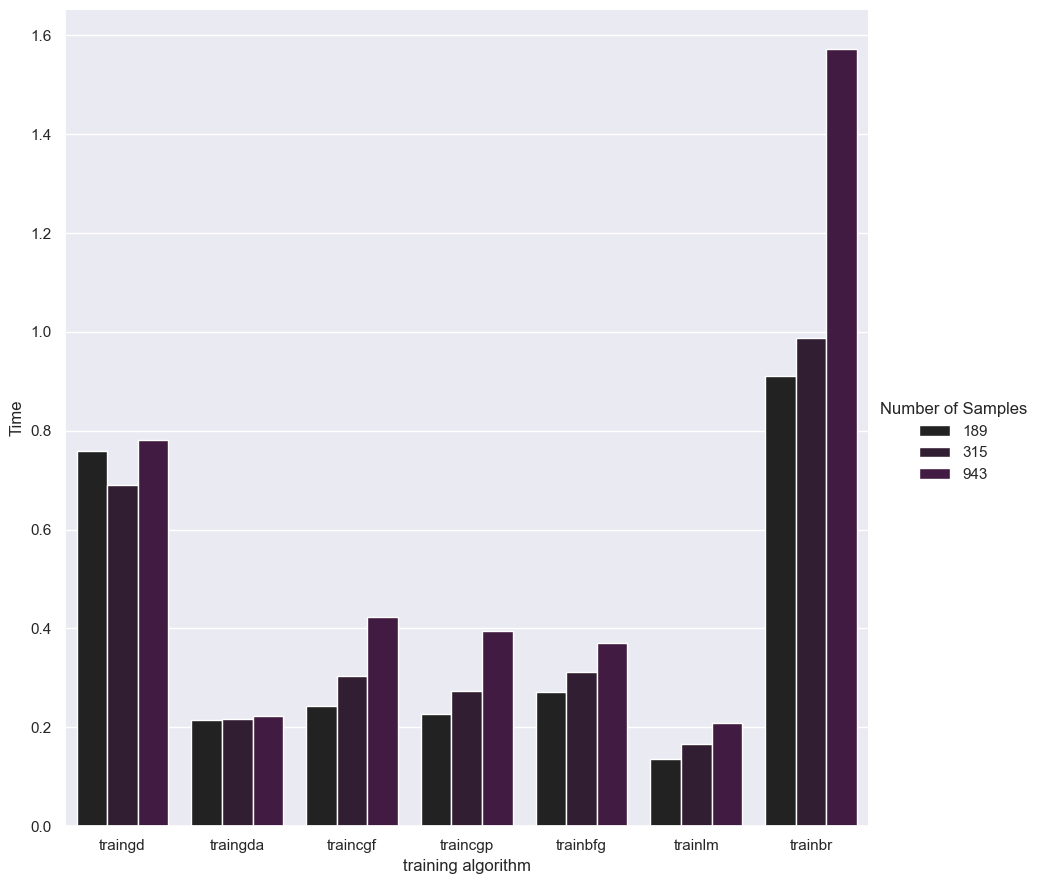
\includegraphics[width=\linewidth]{images/Samples-Time.png}
        \caption{Number of Samples - Time}
    \end{subfigure}
    \begin{subfigure}{0.33\linewidth}
        %\centering
        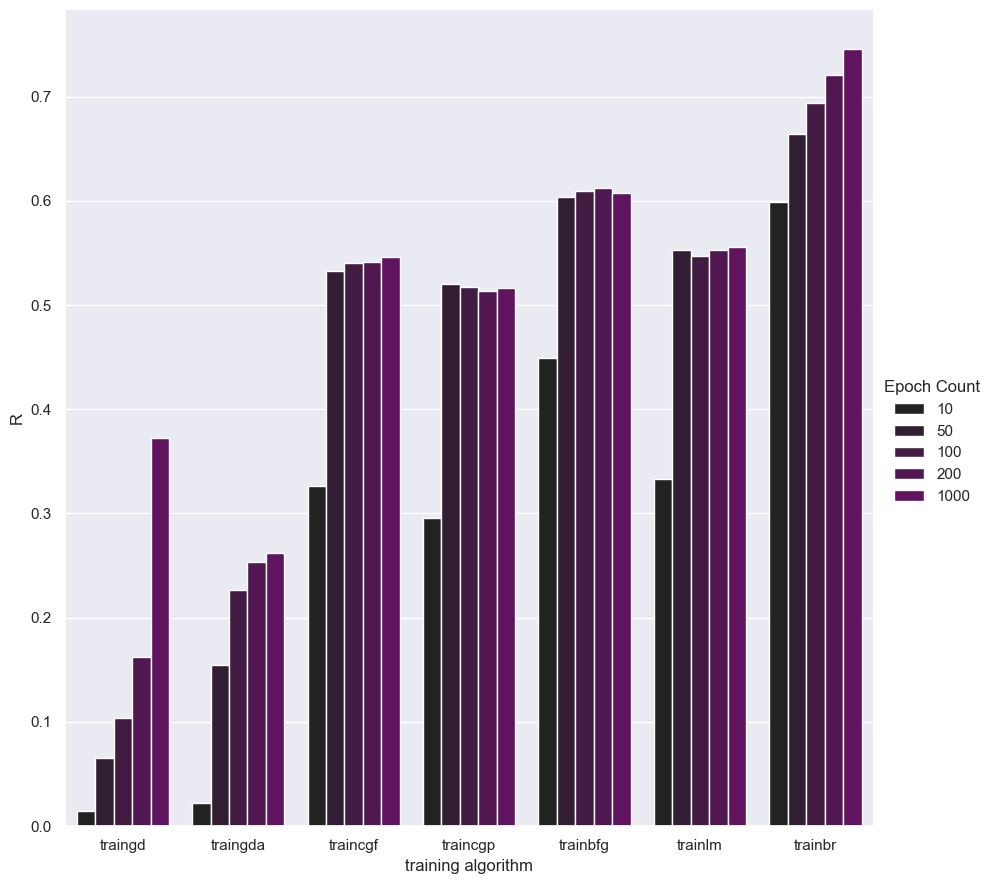
\includegraphics[width=\linewidth]{images/Epochs-R.png}
        \caption{Number of Epochs - R}
    \end{subfigure}
    \begin{subfigure}{0.33\linewidth}
        %\centering
        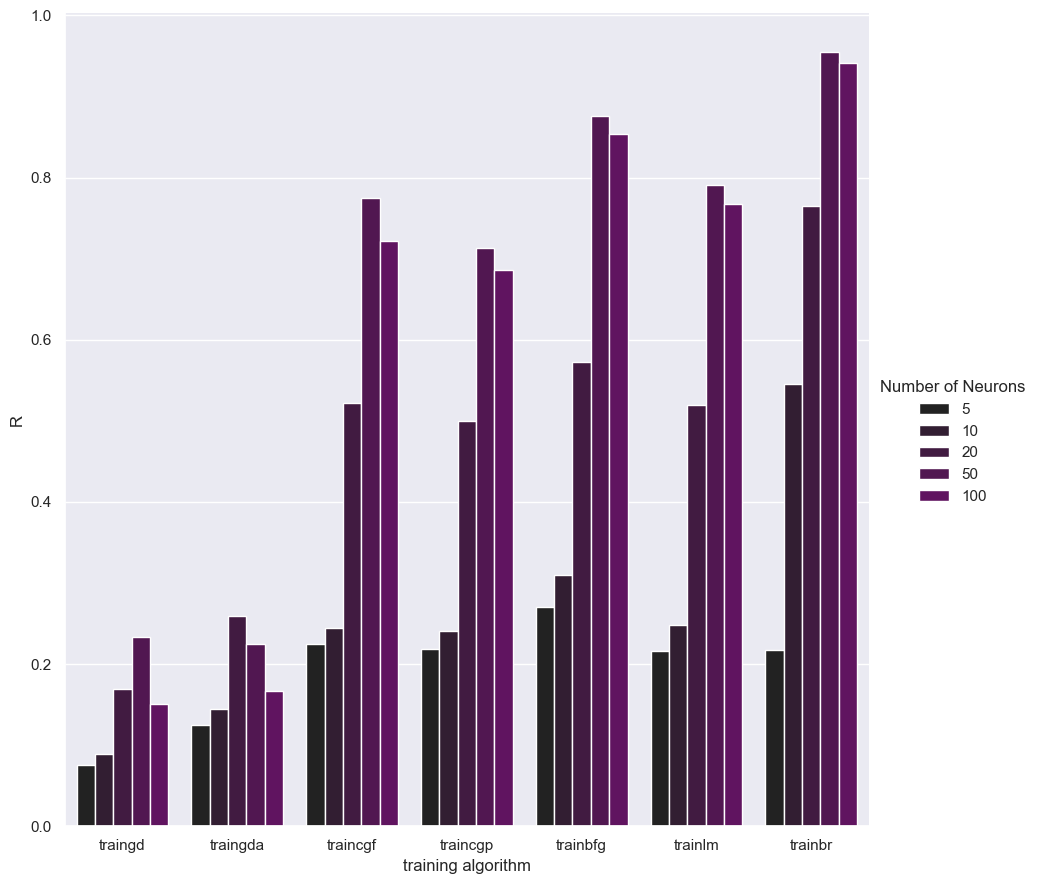
\includegraphics[width=\linewidth]{images/Neurons-R.png}
        \caption{Number of Neurons - R}
    \end{subfigure}
    \begin{subfigure}{0.33\linewidth}
        %\centering
        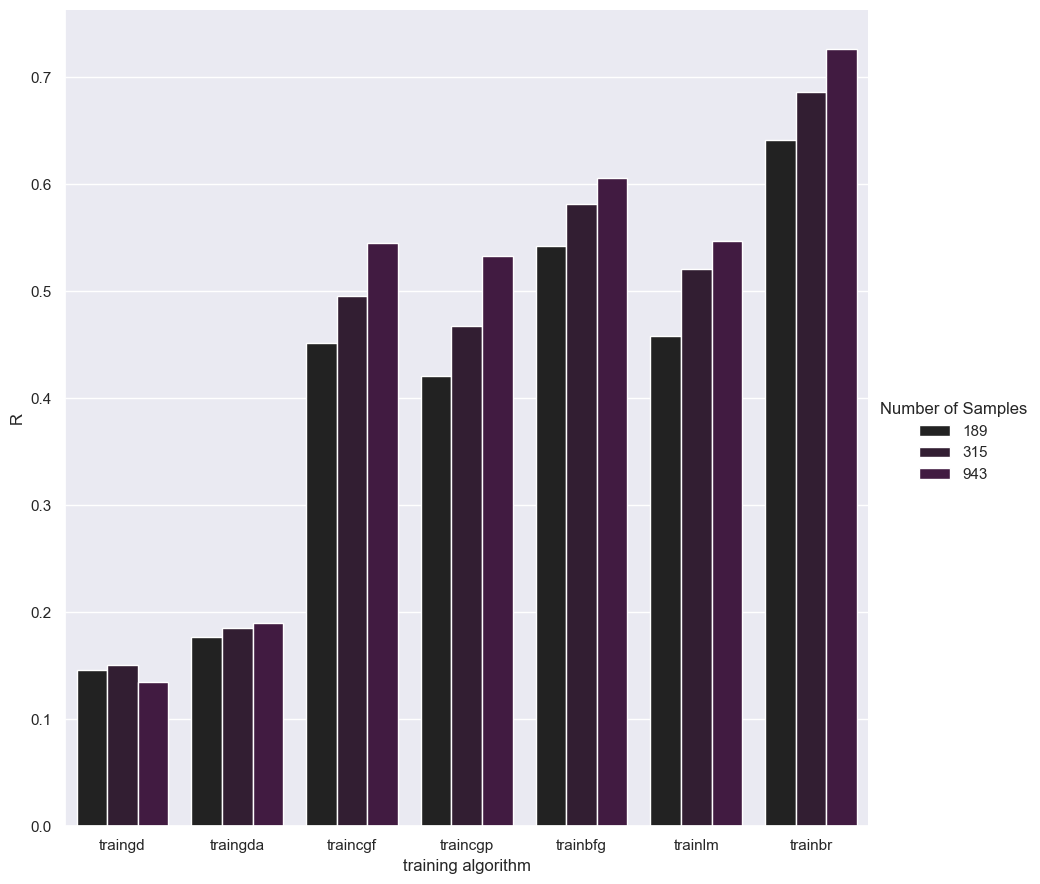
\includegraphics[width=\linewidth]{images/Samples-R.png}
        \caption{Number of Samples - R}
    \end{subfigure}
    
    \caption{ Illustration of performance of training algorithms and the effects of their parameters}
    \label{fig:1}    
    
\end{figure*}

\subsubsection{Performance Evaluation}
As we can observe in Figure 1, Levenberg-Marquardt with Bayesian regularization (\textit{trainbr}) algorithm outperforms all other algorithms in regards to R values. Additionally, Fletcher-Reeves conjugate gradient algorithm (\textit{traincgf)} slightly outperforms Polak-Ribiere conjugate gradient  (\textit{traincgp}), but overall they perform in very similar standards. Gradient descent (\textit{traingd}) and gradient descent with adaptive learning (\textit{traingda}) perform significantly worse than all others, with the latter slightly outperforming the former. The main reason for them underperforming is the fact that they greatly depend on learning rates and in this case it is an arbitrary fixed value. 

In general, gradient descent algorithms tend to fail to converge to local minima when provided with very high learning rates. Additionally, they fail to  
exploit any information of the second order derivatives, thus resulting in an ill-conditioned Hessian matrix. 
Quasi newton methods however do take into account the second order derivative and approximate the Hessian matrix using gradients to update the weights. More specifically, Levenberg-Marquardt addresses this problem by adding $\lambda I$ to the Hessian matrix, which is a positive matrix that makes it possible to inverse the Hessian in a potential case of ill-conditioning. 

As stated previously, Levenberg-Marquardt with Bayesian regularization outperforms all other training algorithms in terms of R values. In Bayesian environments, network weights are determined by a probability distribution, in contrast to focusing on a single weight point. 

\begin{figure}
    \centering
    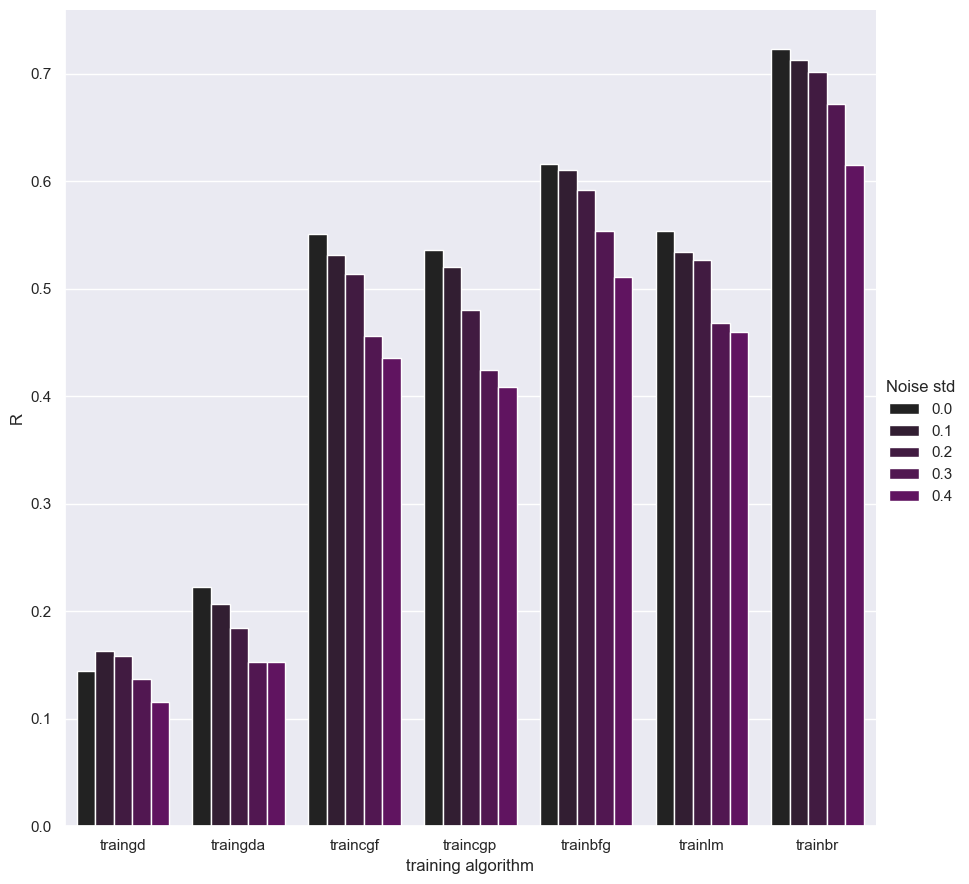
\includegraphics[width=8cm]{images/NoiseStd-R.png}
    \caption{R values of training algorithms when noise is introduced}
    \label{fig:2}
\end{figure}

\subsection{Function Approximation using Regression}
The aim of this exercise was to approximate an unknown linear function using a feedforward neural network. The provided dataset is comprised of 13600 noise-free datapoints and the function that we are trying to approximate is a combination of 5nonlinear functions $f_1,f_2,...,f_5$. Specifically, these functions correspond to $f_1(X1,X2) = T1, f_2(X1, X2) = T2, f_3(X1, X2) = T3, f_4(X1, X2) = T4,  f_5(X1, X2) = T5$ and $T_new$ is $(d_1T1 + d_2T2 + d_3T3 + d_4T4 + d_5T5) / (d_1 + d_2 + d_3 + d_4 + d_5)$. In this case, $(d_1 + d_2 + d_3 + d_4 + d_5)$ correspond to $7 + 6 + 6 + 5 + 5$, since it was required for these numbers to represent our student numbers with the largest digits in decreasing order. 

At first, we merge all the data ($X1$, $X2$ and $Tnew$) into one matrix with 3 rows and 13600 columns. Then we split the original dataset into three new datasets of 1000 points each, thus creating the training, validation and test sets. The training set is used for the training of the model, the test set is used to assess its performance on unseen data whereas the validation set is used optimize the model's performance, since it has data that are independent of the training ones, thus reflecting the model's ability to generalize. The training and test surface are depicted in Figure 3.

\begin{figure*}[]
        \centering
        \begin{subfigure}{0.33\linewidth}
            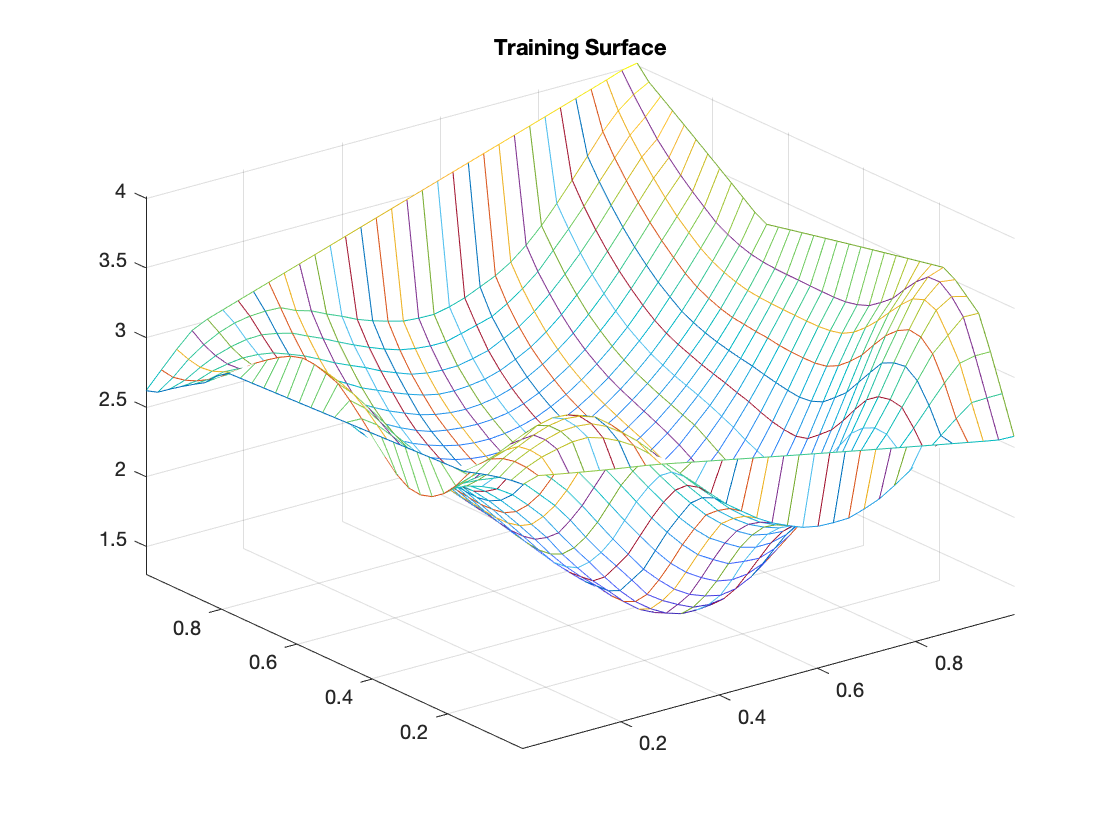
\includegraphics[width=\linewidth]{images/training.png}
            \caption{Training Surface}
        \end{subfigure}
        \begin{subfigure}{0.33\linewidth}
            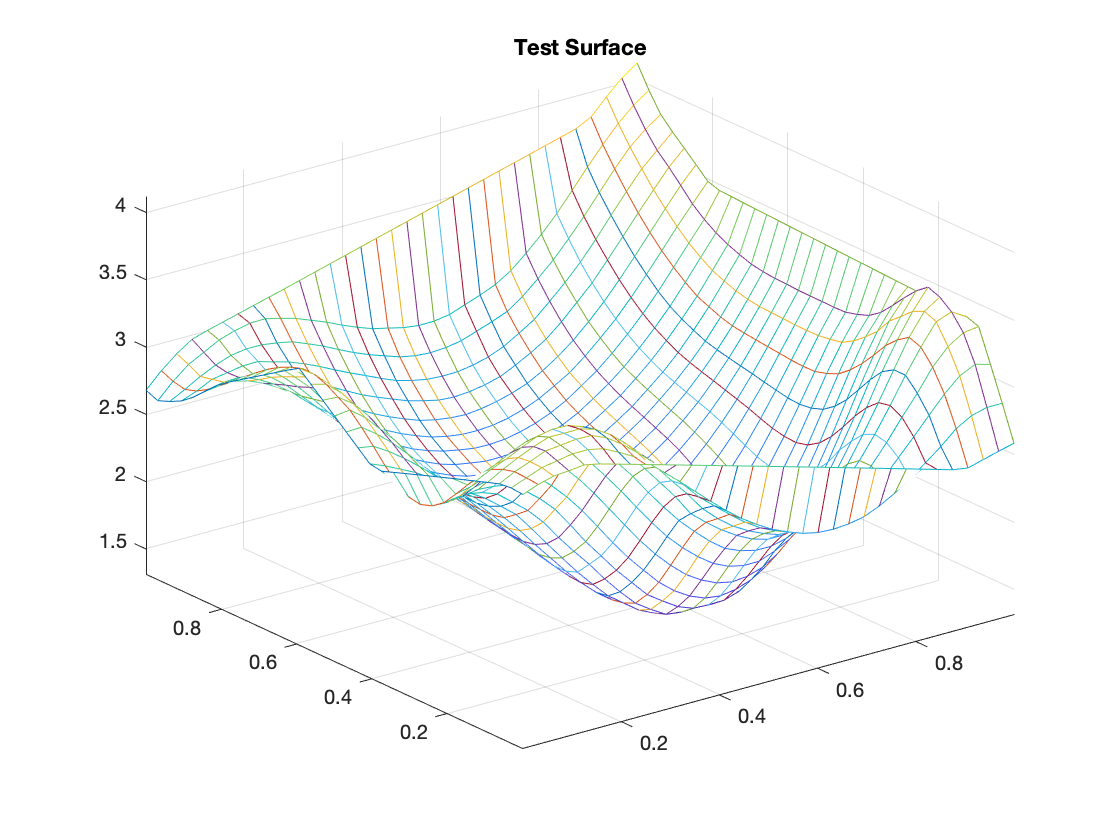
\includegraphics[width=\linewidth]{images/test.png}
            \caption{Test Surface}
        \end{subfigure}
        \caption{Personal regression training and test surfaces}
        \label{fig:3}
\end{figure*}

\begin{figure}
    \centering
    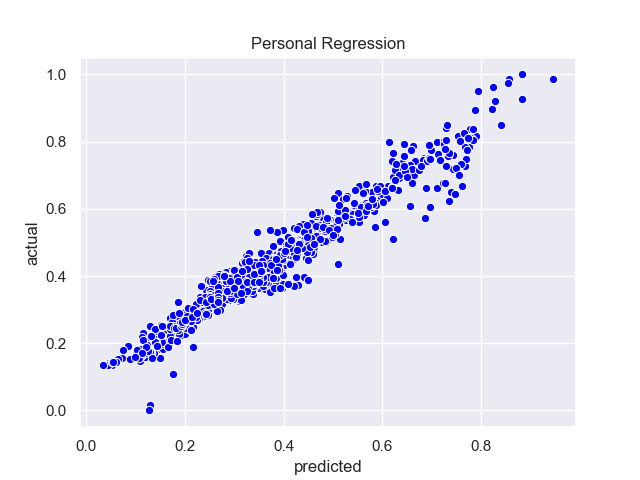
\includegraphics[width=8cm]{images/regression.png}
    \caption{Predicted against actual values for the regression task}
    \label{fig:4}
\end{figure}


\subsubsection{Training and Performance}
In order to define the most suitable model for this task the network is trained with different algorithms and different numbers of neurons for each layer. It was considered sufficient to only use one hidden layer for this simple regression task, since, as mentioned earlier, it is possible to approximate any (continuous) function using only one hidden layer, based on the universal approximation theorem. The number of neurons for this hidden layer varied from 5, to 10 and 20. The algorithm that performs the best is Levenberg-Marquardt with an architecture of 20 neurons and the performance is, as requested, evaluated on the test set for 10 runs of each algorithm using MSE. The results are presented in Table 1 whereas the predicted against actual values are shown in Figure 4.  

\begin{table*}
\centering
\begin{tabular}[t]{l l l l l l l}
\toprule 
 Neurons & trainlm & traingda & traincgf & traincgp & trainbfg & traingd \\
\midrule
 5 & 0.032 & 0.026 & 0.012 & 0.014 & 0.013 & 0.139\\
 10 & 0.0011 & 0.024 & 0.0027 & 0.0039 & 0.0015 & 0.088 \\
 20 & \textbf{2.39e-05}  & 0.021 & 0.0023 & 0.0017 & 0.00023 & 0.059 \\
\bottomrule
\end{tabular}
\label{tbl:1}
\caption{MSE for the MLP with number of neurons over 10 runs in the test set for different training algorithms}
\label{1}
\end{table*}

\section{Recurrent Neural Networks}
\subsection{Hopfield Network}
Hopfield networks are a form of recurrent neural networks that work in associative memory and are designed to store patterns. A Hopfield network has one set of fully interconnected neurons that can have two states, either $S_i = 1$ or $S_i = -1$. The output from time $t$ is used as an input at time $t+1$, thus letting the network to dynamically evolve in a synchronous way. Eventually, the network reaches a stable state, which is called an \textit{atractor} and the values of the neurons stop being updated. Their ability to work in associative memory means that Hopfield networks are not susceptible to noise since they can retrieve values that are associated with the patterns they have already stored. Updates can be either asynchronous or synchronous, the former meaning that only one unit is updated at a time and the latter meaning that all units are updated at the same time. An issue that arises in such networks is that it is possible they might store patterns that are not useful and are unwanted, which are called spurious states. 

In the first part of this exercise we create a Hopfield network with attractors $T = [1\;\;1 ; -1-1 ; 1-1]$. The steps are either 15 or 25 and the number of simulations vary from 5, to 10 and 25. After running various experiments, it was observed that when increasing the number of iterations from 10 and higher usually results in reaching the attractors. The number of real attractors is actually 4, since we also have $[-1\;\; 1]$, which is added by the model. The results in these iterations are shown in Figure 5.

\begin{figure*}[]

    \begin{subfigure}{0.33\linewidth}
        %\centering
        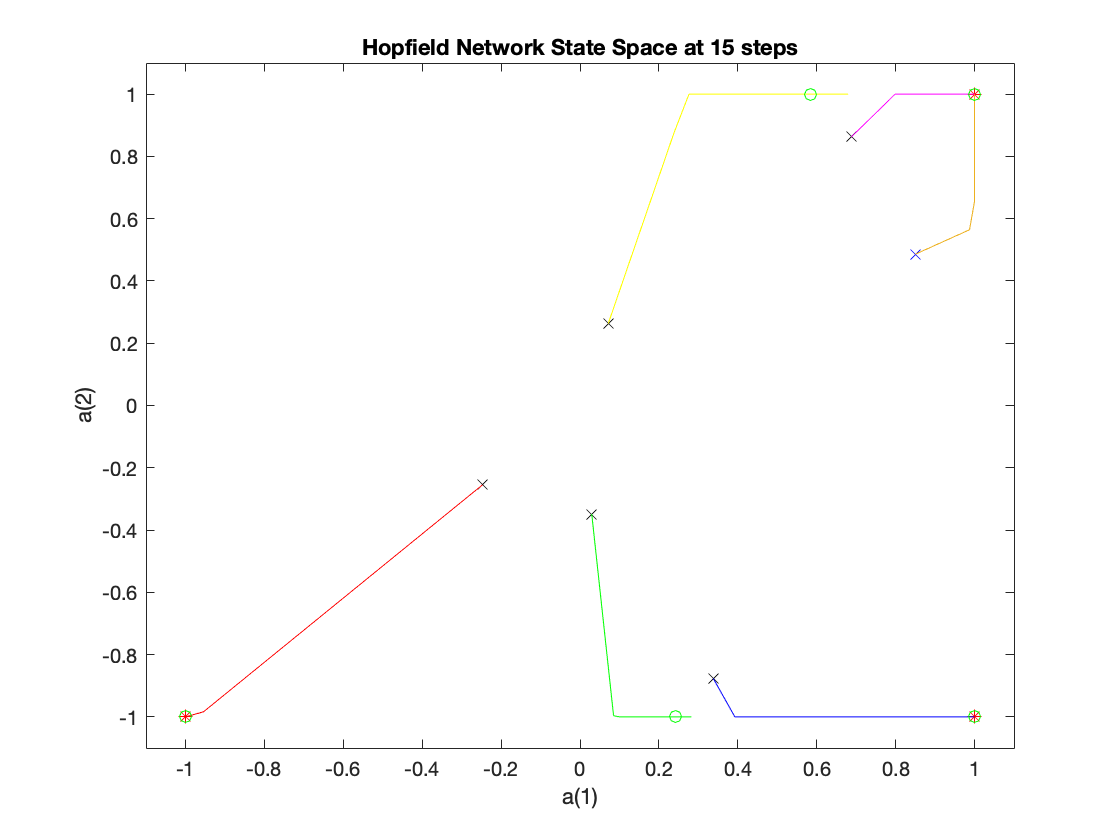
\includegraphics[width=\linewidth]{images/hopfield1_15steps_5sims.png}
        \caption{15 steps 5 simulations}
    \end{subfigure}
    \begin{subfigure}{0.33\linewidth}
        %\centering
        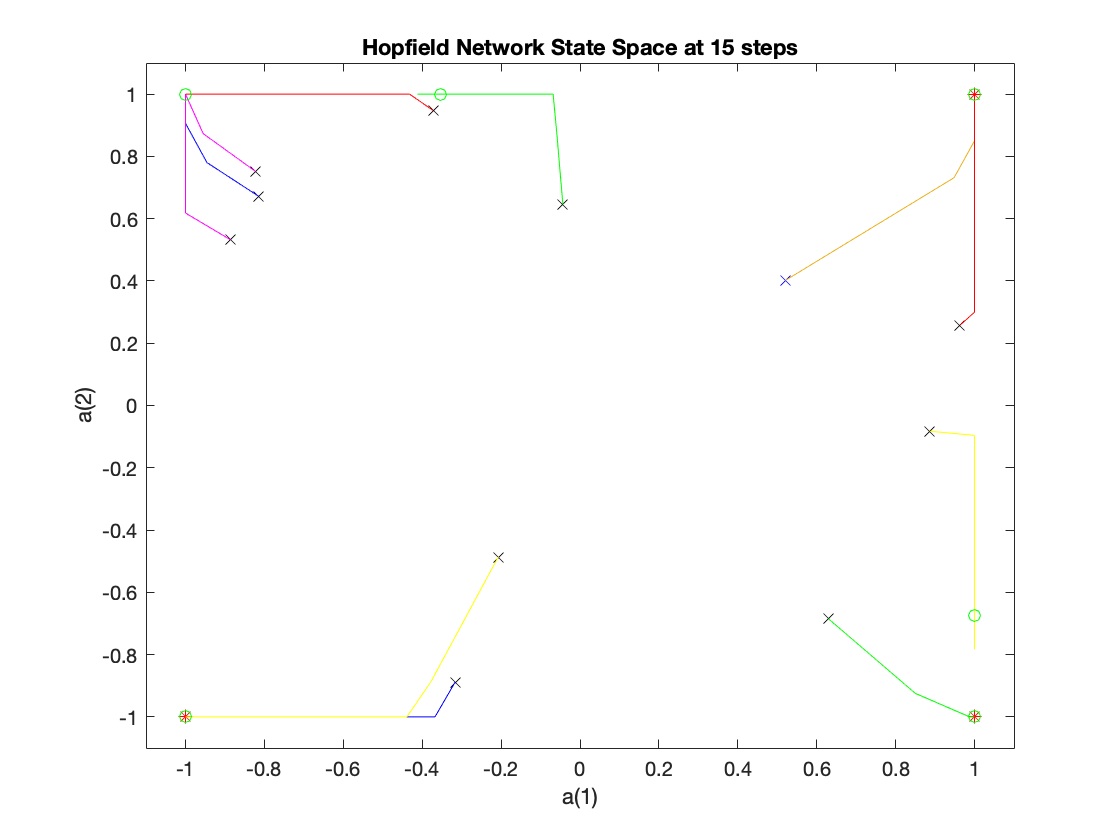
\includegraphics[width=\linewidth]{images/hopfield1_15steps_10sims.png}
        \caption{15 steps 10 simulations}
    \end{subfigure}
    \begin{subfigure}{0.33\linewidth}
        %\centering
        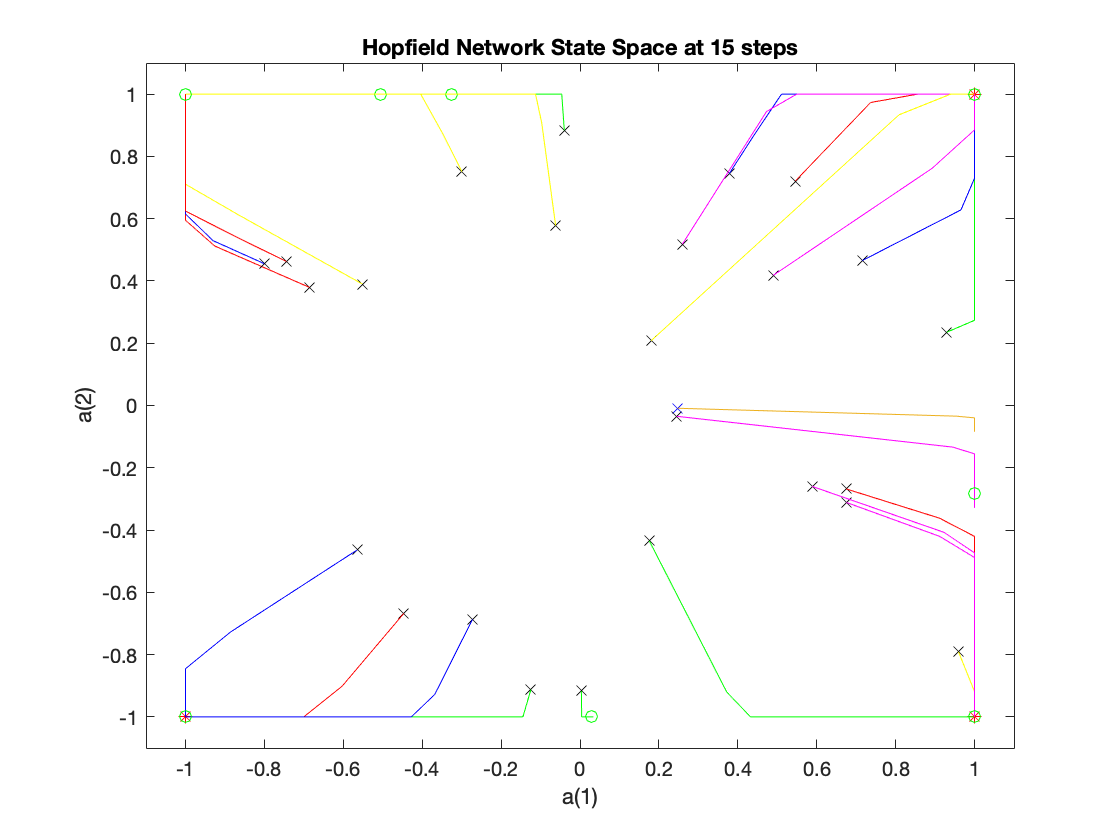
\includegraphics[width=\linewidth]{images/hopfield1_15steps_25sims.png}
        \caption{15 steps 25 simulations}
    \end{subfigure}
    \begin{subfigure}{0.33\linewidth}
        %\centering
        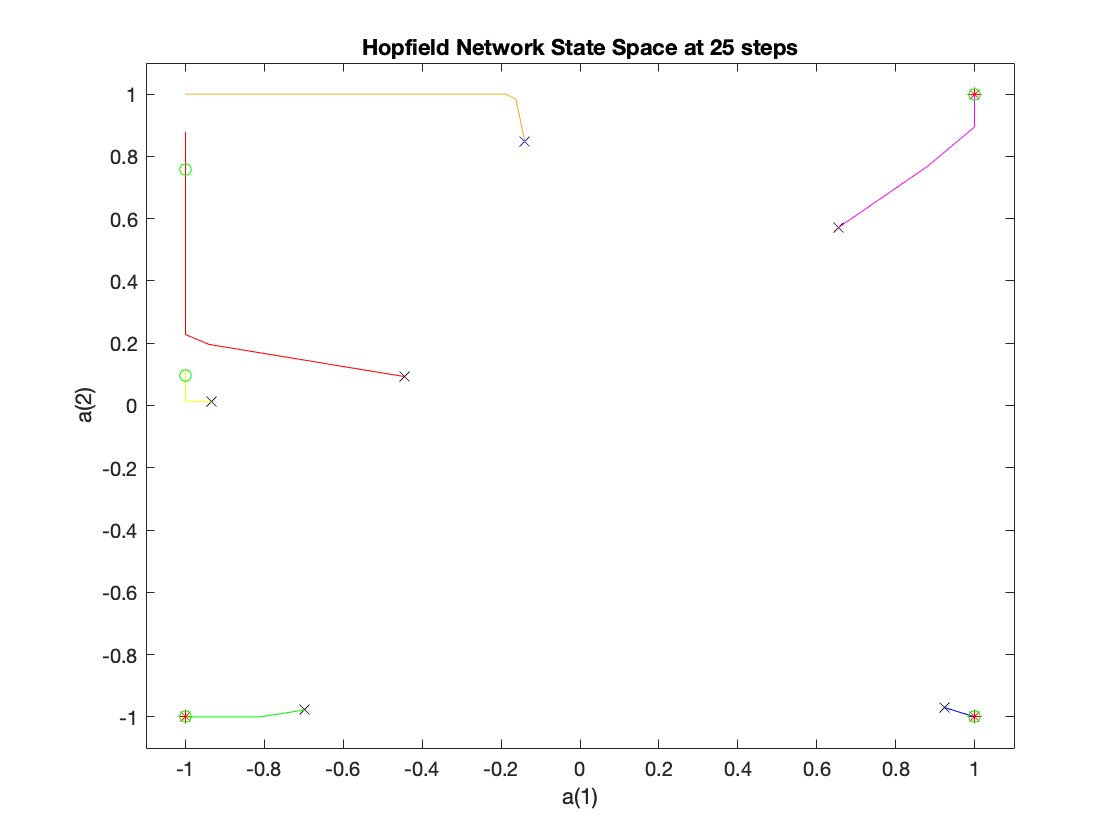
\includegraphics[width=\linewidth]{images/hopfield1_25steps_5sims.png}
        \caption{25 steps 5 simulations}
    \end{subfigure}
    \begin{subfigure}{0.33\linewidth}
        %\centering
        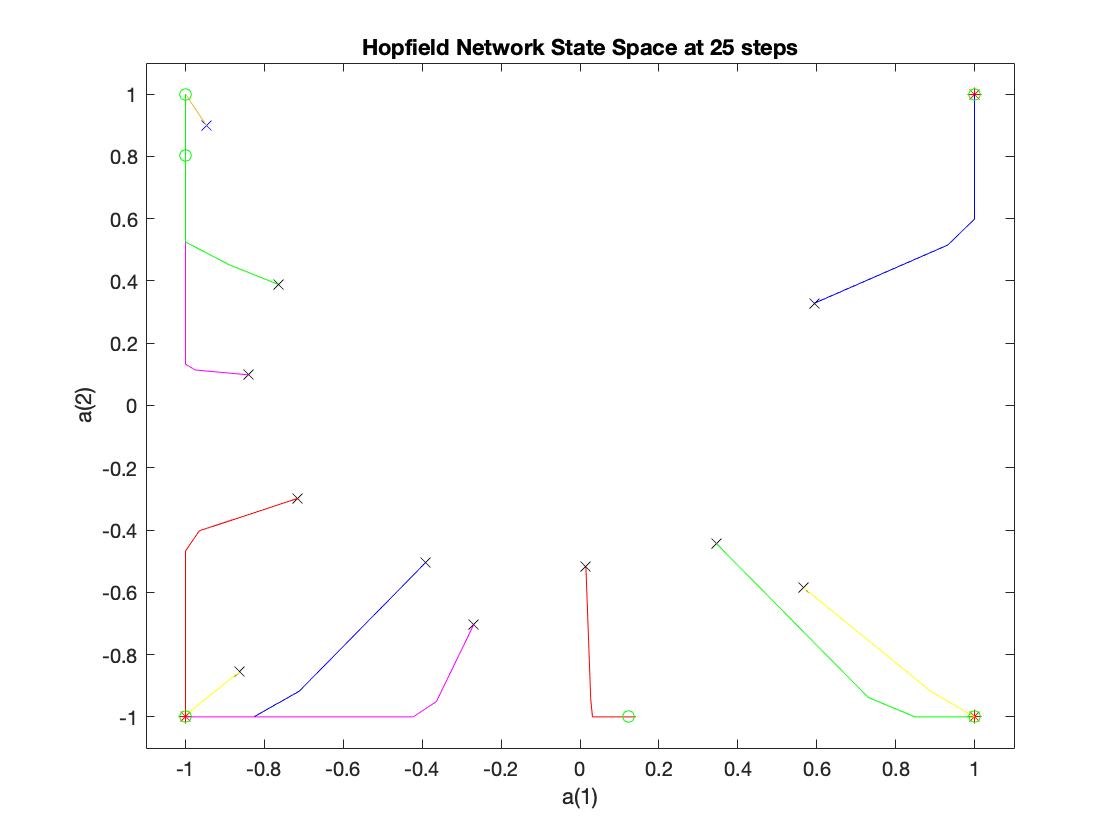
\includegraphics[width=\linewidth]{images/hopfield1_25steps_10sims.png}
        \caption{25 steps 10 simulations}
    \end{subfigure}
    \begin{subfigure}{0.33\linewidth}
        %\centering
        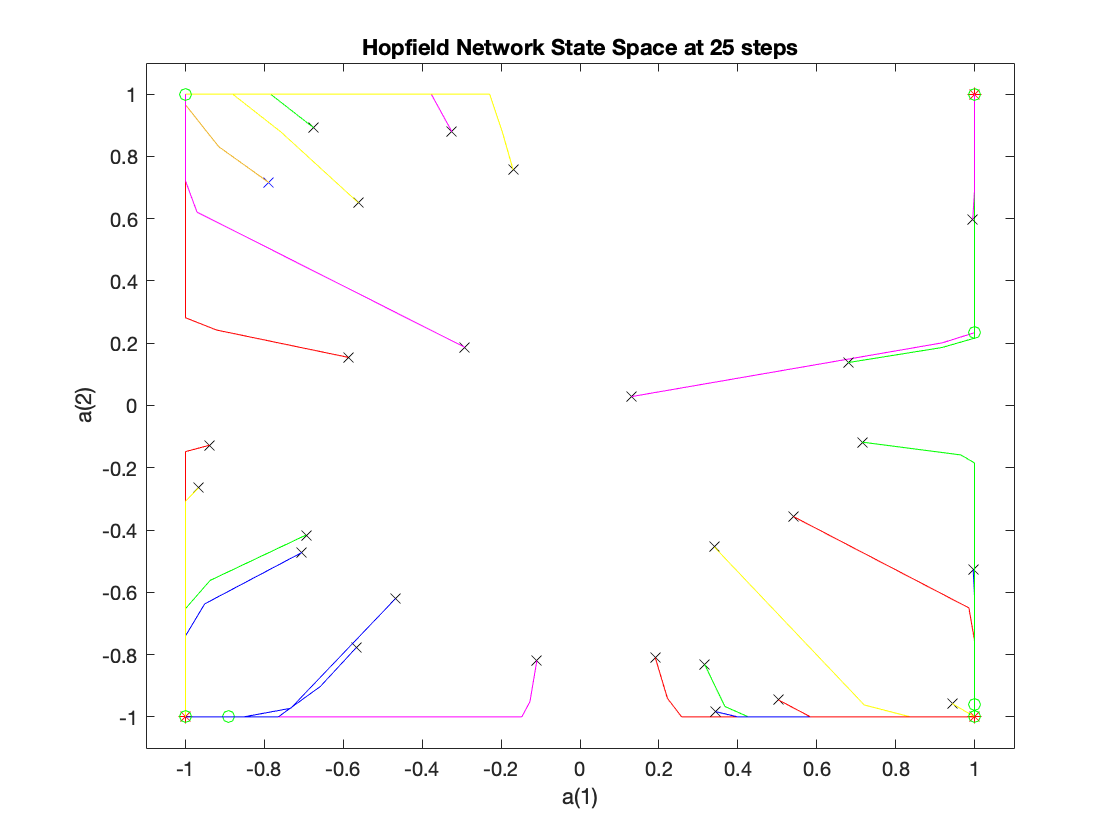
\includegraphics[width=\linewidth]{images/hopfield1_25steps_25sims.png}
        \caption{25 steps 25 simulations}
    \end{subfigure}
    
    \caption{ Illustration of Hopfield network State Space}
    \label{fig:5}    
    
\end{figure*}

When executing the scripts \textit{rep2} and \textit{rep3} we notice that in both cases there exist spurious states and also that symmetrical points to the patterns are converted to attractors. This is illustrated in Figure 6.

\begin{figure*}[]
        \centering
        \begin{subfigure}{0.33\linewidth}
            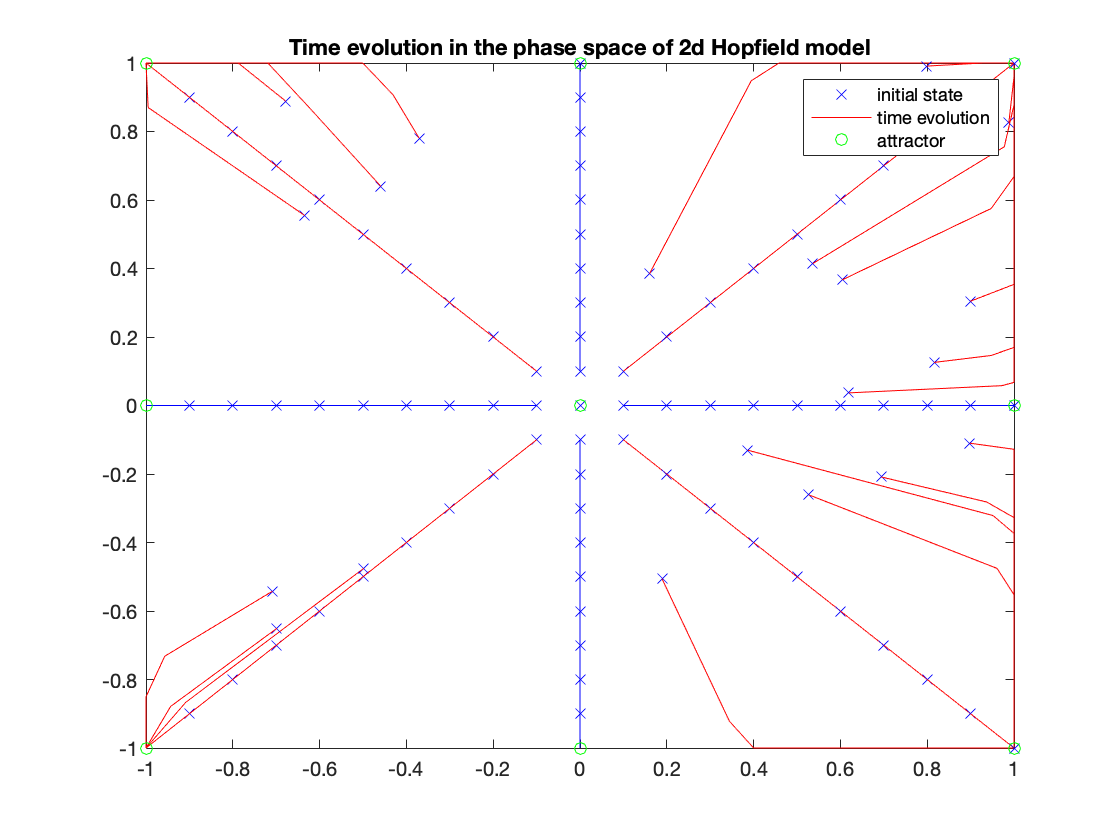
\includegraphics[width=\linewidth]{images/hopfield1_rep2.png}
            \caption{rep2}
        \end{subfigure}
        \begin{subfigure}{0.33\linewidth}
            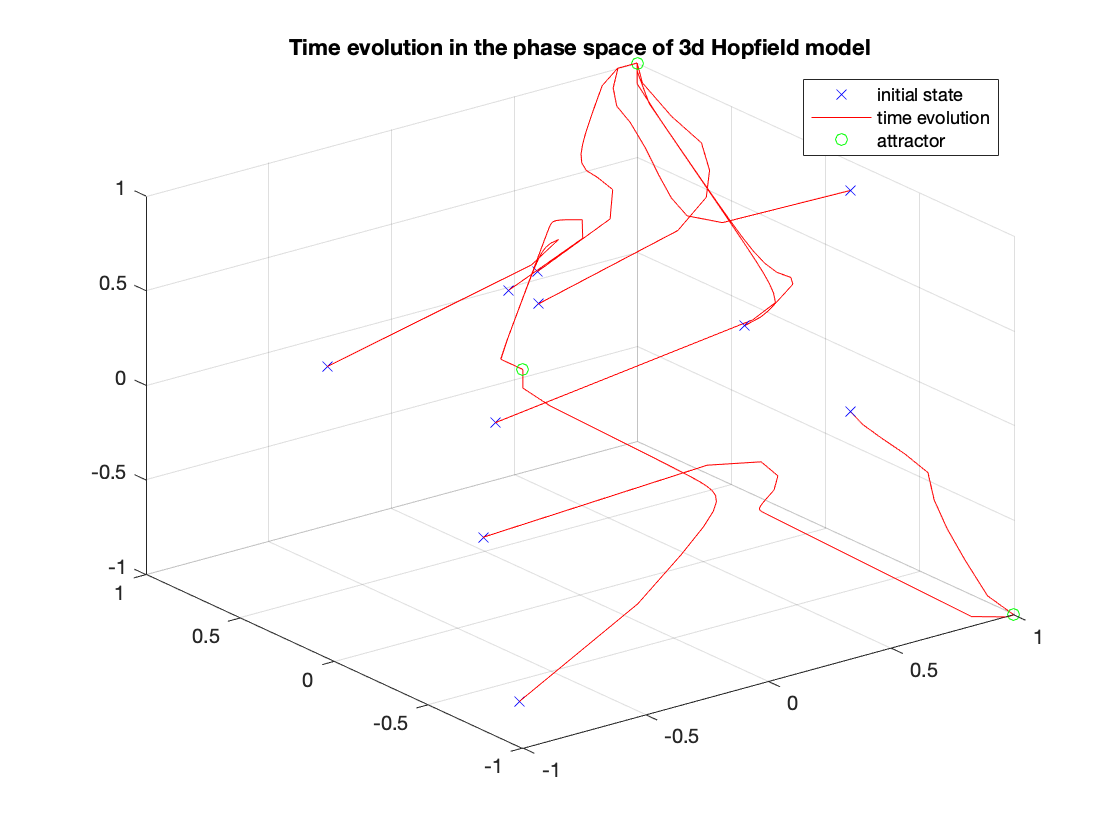
\includegraphics[width=\linewidth]{images/hopfield1_rep3.png}
            \caption{rep3}
        \end{subfigure}
        \caption{Execution of rep2 and rep3 scripts}
        \label{fig:6}
\end{figure*}

In the final part of this exercise we create a Hopfield network which has as attractors the handwritten digits from 0 to 9. The number of simulations was varied from 5 to 10 and 30 and the amount of noise from 1 to 5 and 10. For low values of noise (1) we do not notice any significant differences, therefore the results that are shown in Figure 7 are only the interesting and meaningful ones, where noise varies from 5 to 10. 

\begin{figure*}[]
    \begin{subfigure}{0.32\linewidth}
        %\centering
        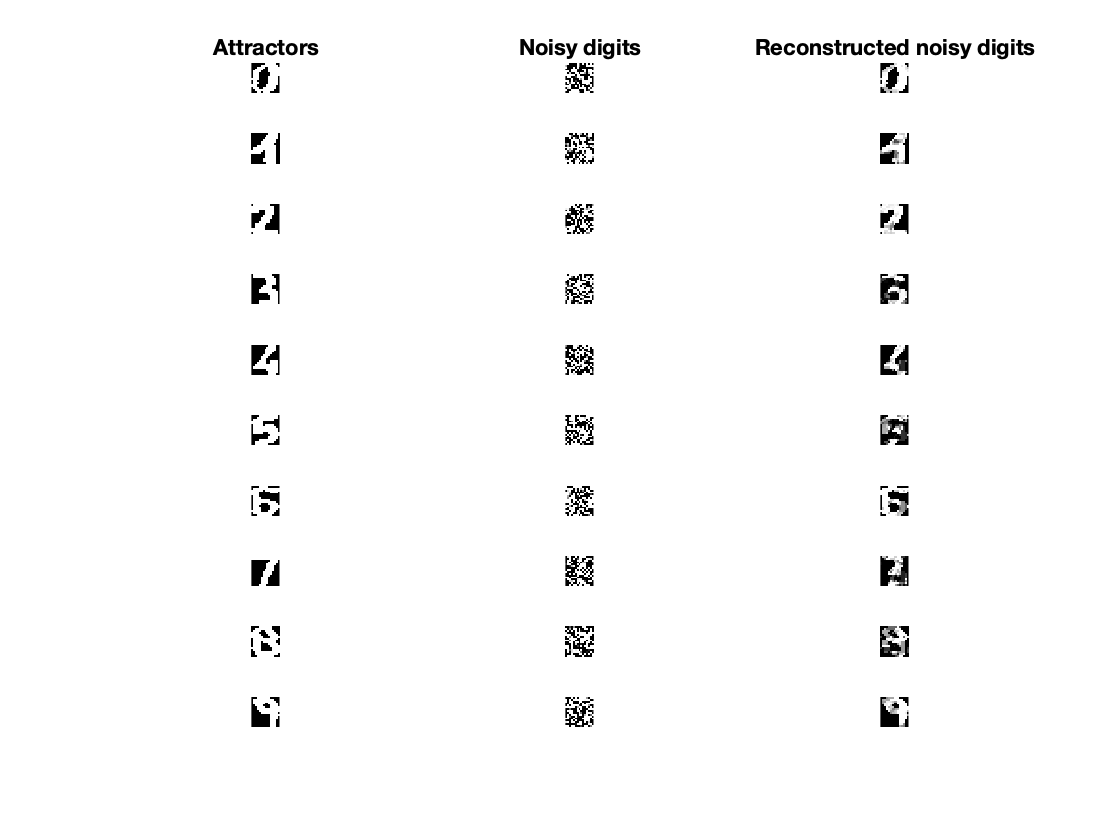
\includegraphics[width=\linewidth]{images/noise5_iter5.png}
        \caption{Noise 5 Iterations 5}
    \end{subfigure}
    \begin{subfigure}{0.32\linewidth}
        %\centering
        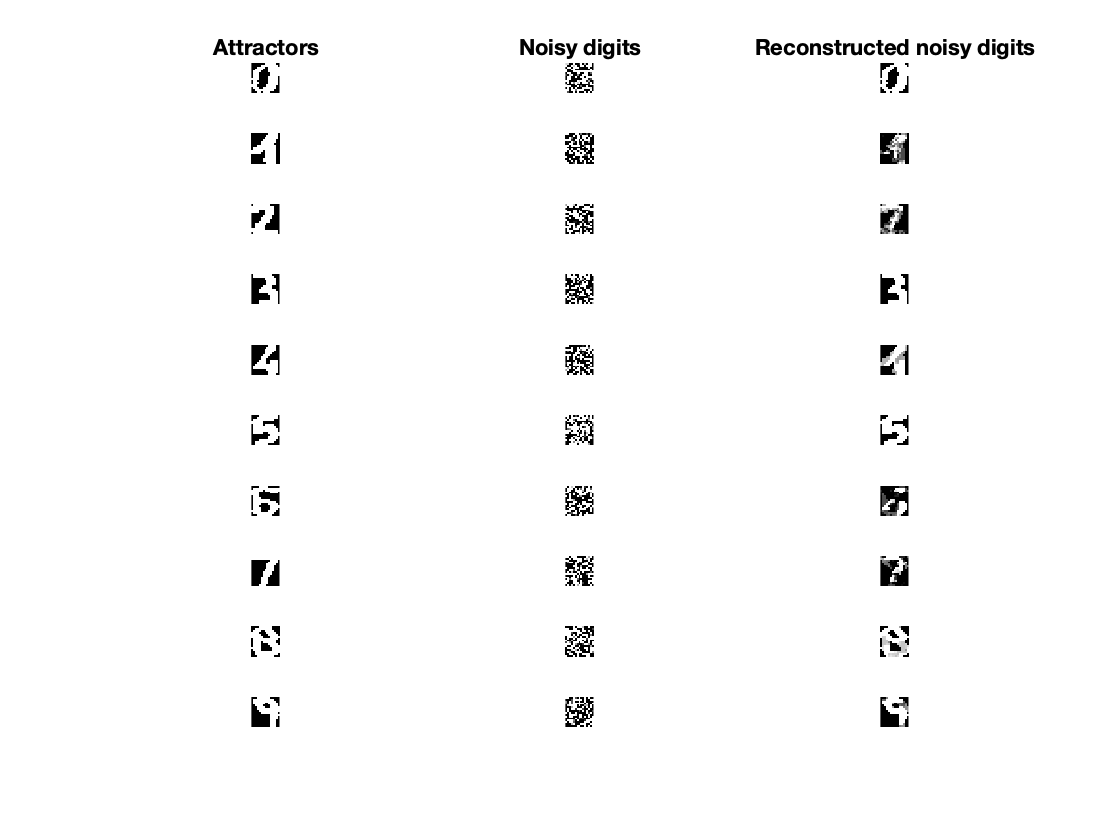
\includegraphics[width=\linewidth]{images/noise5_iter10.png}
        \caption{Noise 5 Iterations 10}
    \end{subfigure}
    \begin{subfigure}{0.32\linewidth}
        %\centering
        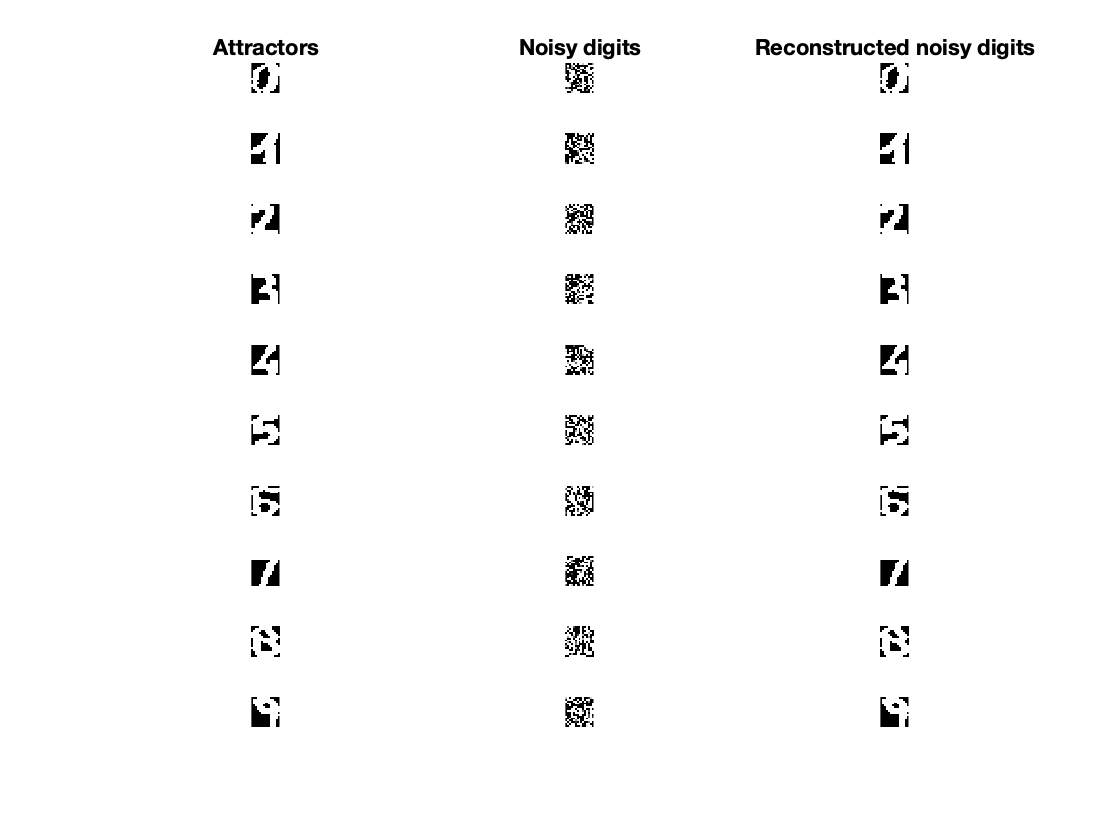
\includegraphics[width=\linewidth]{images/noise5_iter30.png}
        \caption{Noise 5 Iterations 30}
    \end{subfigure}
    \begin{subfigure}{0.32\linewidth}
        %\centering
        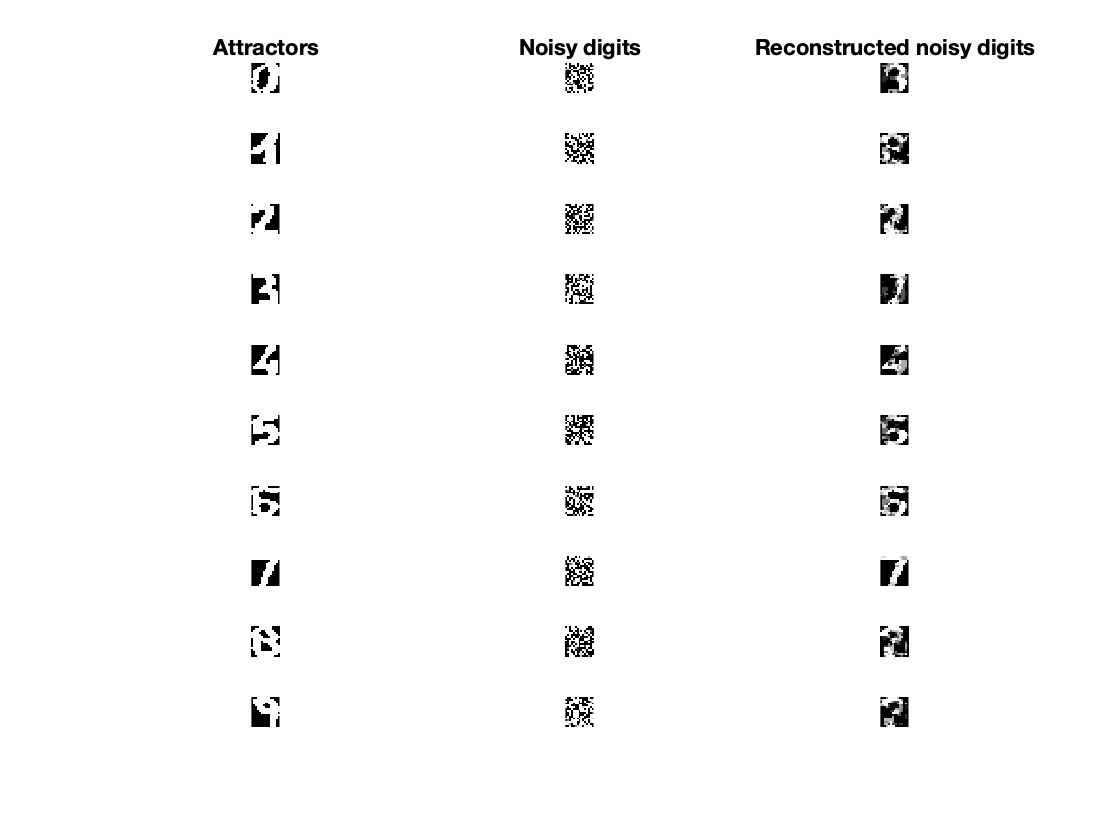
\includegraphics[width=\linewidth]{images/noise10_iter5.png}
        \caption{Noise 10 Iterations 5}
    \end{subfigure}
    \begin{subfigure}{0.32\linewidth}
        %\centering
        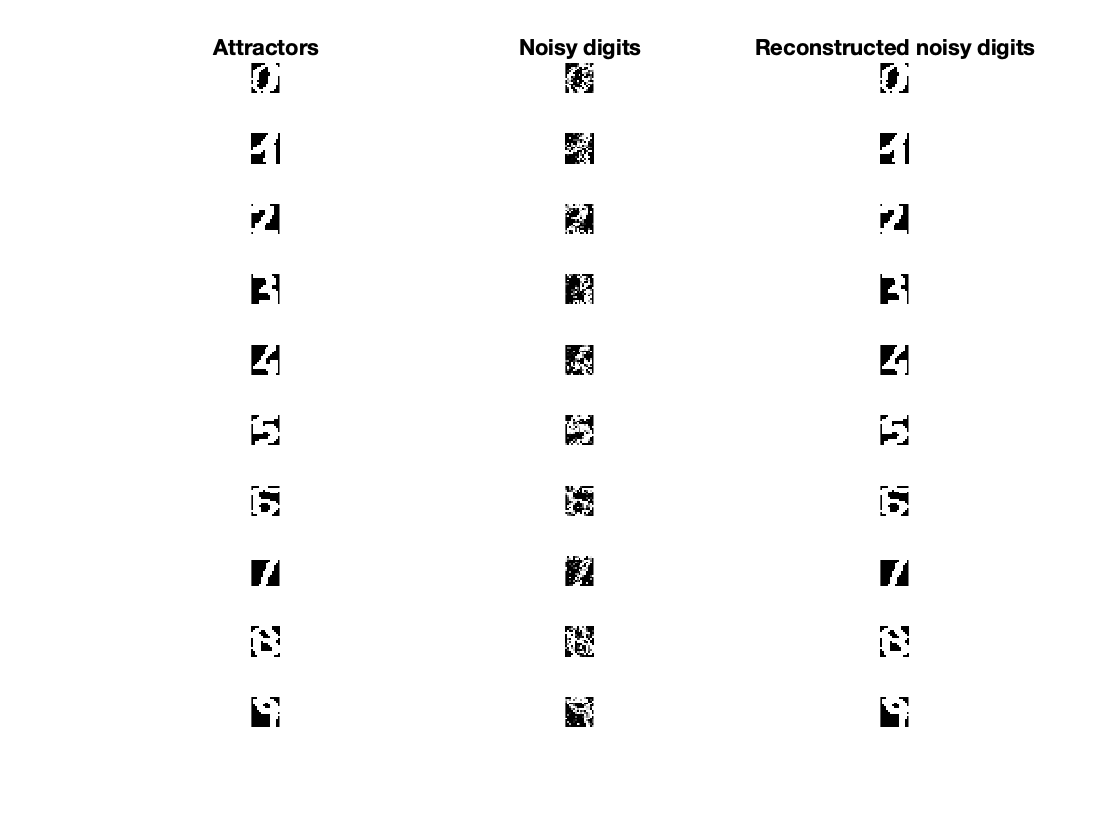
\includegraphics[width=\linewidth]{images/noise1_iter10.png}
        \caption{Noise 10 Iterations 10}
    \end{subfigure}
    \begin{subfigure}{0.32\linewidth}
        %\centering
        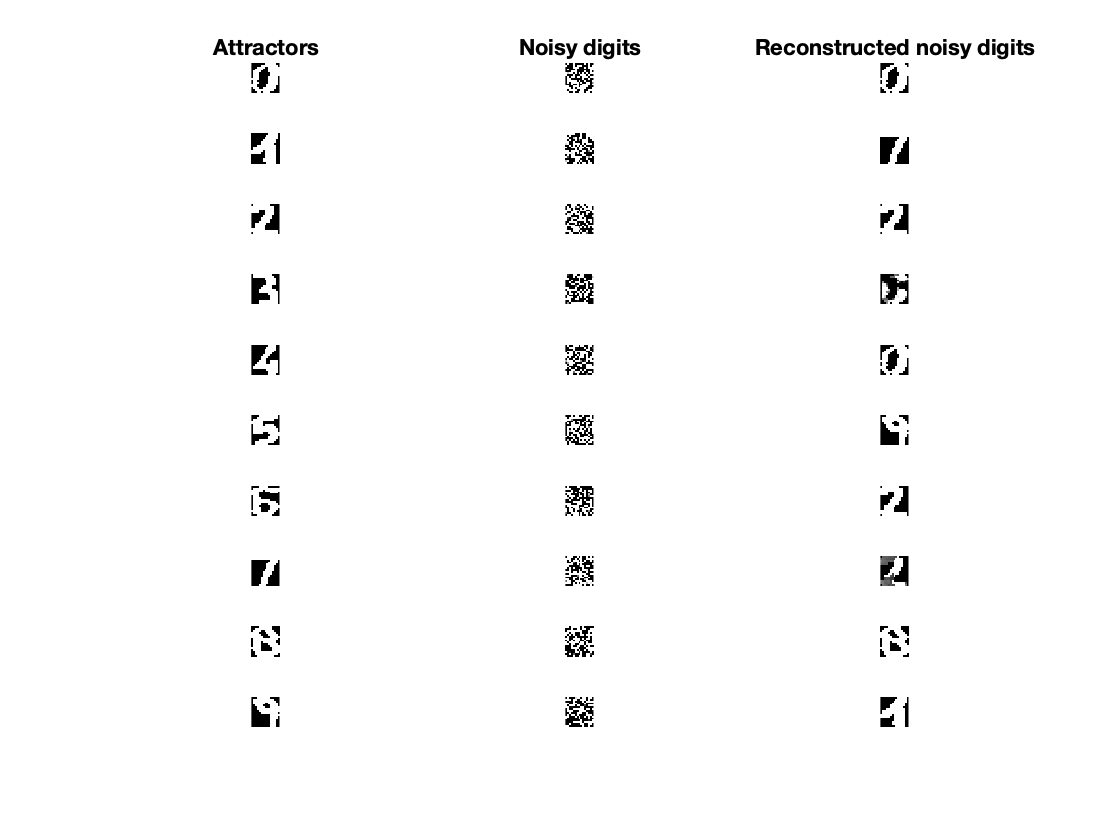
\includegraphics[width=\linewidth]{images/noise10_iter30.png}
        \caption{Noise 10 Iterations 30}
    \end{subfigure}
    
    \caption{Attractors, noisy digits and Reconstructed digits}
    \label{fig:7}    
    
\end{figure*}

\subsection{Long Short-Term Memory Networks}
\subsubsection{Time Series Prediction}
The aim of this exercise is to train two different networks using the Santa Fe data set for Time Series prediction. This data set is acquired from a chaotic laser and consists of 1000 data points. The networks that are trained are a) a recurrent multi-layer perceptron (MLP) and b) a Long Short-Term Memory Network (LSTM).   
\subsubsection{Multi-layer perceptron}
The MLP has one hidden layer is trained in a feedforward fashion. Considering the fact that the model can only predict one step ahead in time, since it takes the predicted value from the previous timestep and includes it in the input of the next timestep, we use the network as a recurrent one. We format the data using \textit{getTimeSeriesTrainData} command and then we experiment with different numbers of neurons and lag. In Figure 8 we can see the performance of the MLP for a lag $p = 5$ and number of hidden neurons 100.

\begin{figure}[h!]
    \centering
    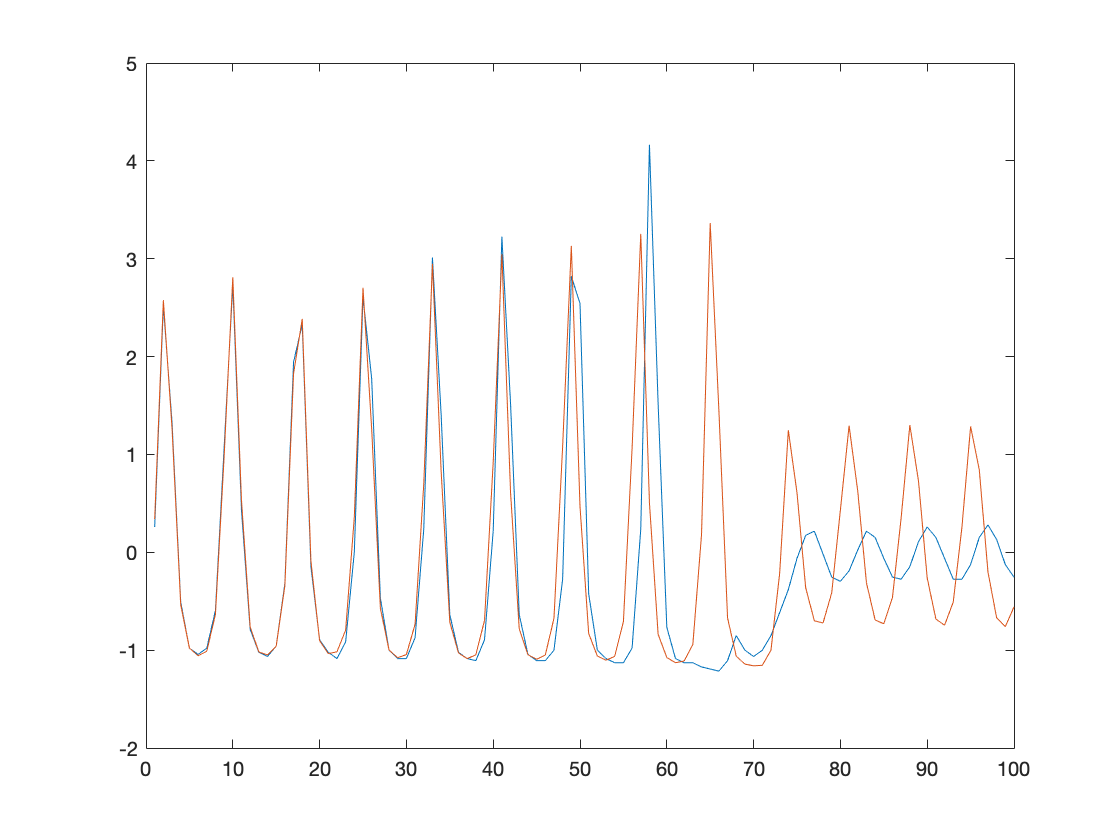
\includegraphics[width=8cm]{images/mlp_perf.png}
    \caption{MLP performance}
    \label{fig:8}
\end{figure}

\subsubsection{Long Short-Term Memory Network}
LSTMs are artificial recurrent neural networks that unlike standard feedforward neural networks have feedback connections. LSTMs can keep track of long-term dependencies in the input sequences and a typical architecture consists of a \textit{cell}, which corresponds to the LSTM's memory, and three regulators (gates), namely the forget gate $f$, the input gate $i$ and the output gate $o$. The above gates act as regulators in the sense that they regulate the information that flows to the cell. The input and output gates are responsible for controlling the input and output values that flow through the cell and the forget gate for controlling the information that remain in the cell. 
The LSTM is trained using \textit{adam} algorithm for 1000 epochs with an initial learning rate that varied from 0.001 to 0.003 and 0.005, since small learning rates perform better than large ones. The drop factor varies from 01. to 0.3 and 0.5, according to the learning rate, since we don't want to greatly decrease an already rather small learning rate. Finally, the drop period is set to 150 to avoid fast and further decrease of the learning rate. When first generate the predictions of the model and then compare them with the test data we notice a high RMSE score. In contrast, when we update the network at each prediction and then input previous predictions to the function, the results are clearly improved. Figure 9 illustrates this situation, where the RMSE score decreases from 70.02 to 4.96.
Overall, LSTMs are the preferred option when it comes to time series prediction, since they are able to store information and update their state based on this information they have stored. In general, recurrent neural networks and, in this case, especially LSTMs do not have to perform backpropagation, therefore they are more effective whenever an application needs to perform time series predictions.


\begin{figure*}[]
    \centering
    \begin{subfigure}{0.4\linewidth}
    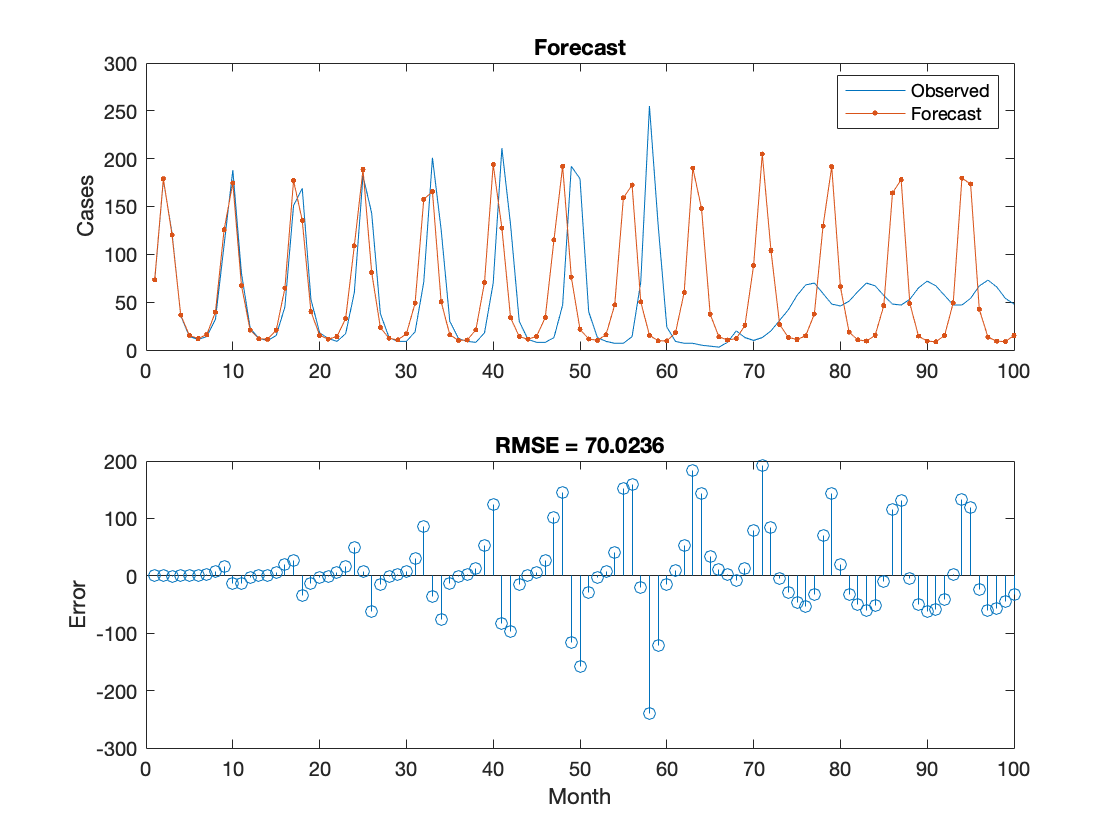
\includegraphics[width=\linewidth]{images/lstm_Ypred.png}
    \end{subfigure}
    \begin{subfigure}{0.4\linewidth}
    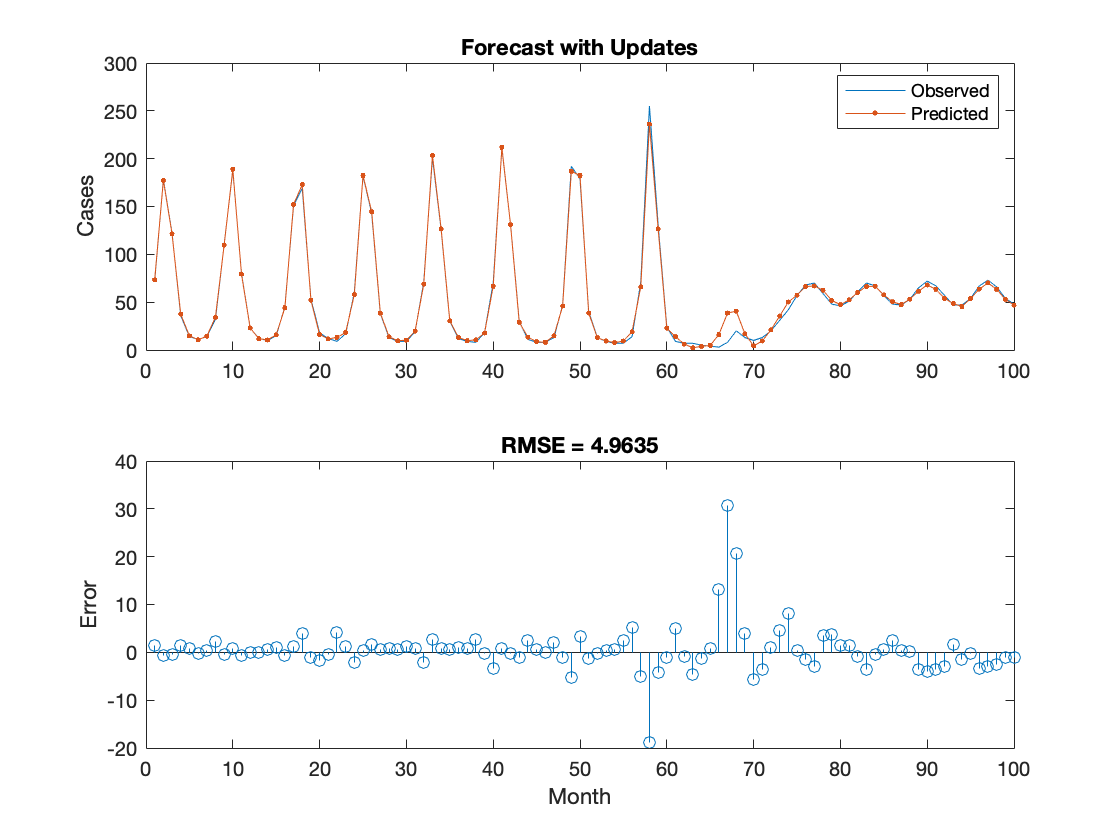
\includegraphics[width=\linewidth]{images/lstm_XTest.png}
    \end{subfigure}
    \caption{LSTM pred and test}
    \label{fig:9}
\end{figure*}

\section{Deep Feature Learning}
\subsection{Principal Component Analysis on Handwritten Digits}
Principal Components Analysis (PCA) aims to map a given vector of a certain dimensional space to a lower vector in a lower dimensional space. The first step is to calculate the mean of the dataset and then subtract it from each datapoint. The next step is to compute the covariance matrix, which expresses the difference between the observations and the mean. We then calculate the eigenvectors and the eigenvalues for this covariance matrix, which are called principal components. 
In this  particular exercise, the task is to perform PCA on a dataset of handwritten images of the digit 3, obtained by the US Postal Service database. Each image is of size $16 \times 16$ and they construct a $500 \times 256$ matrix, where each line is an image of 3 with the aforementioned size that is expanded to a 256 dimensional vector. We first compute the mean and then compute the covariance matrix for the dataset of 3s. Then we plot the eigenvalues, shown in Figure 10. Next step is to compress the dataset and project it into 4 principal components. This is achieved by multiplying the data matrix with a matrix that contains the first 4 eigenvectors in our case (in general for $q$ principal components it contains the first $q$ eigenvectors). Finally, we reconstruct the image to 1, 5, 10, 20, 50 and 256 components. The mean and the reconstructed images are shown in Figure 11. 
As the number of $q$ principal components increases, the reconstruction error decreases, which is expected, since we are using more principal components. This is understandable considering the fact that the components contain a higher amount of variance. Figure 12 illustrates the reconstruction loss which decreases as principal components increase.

\begin{figure}[h]
    \centering
    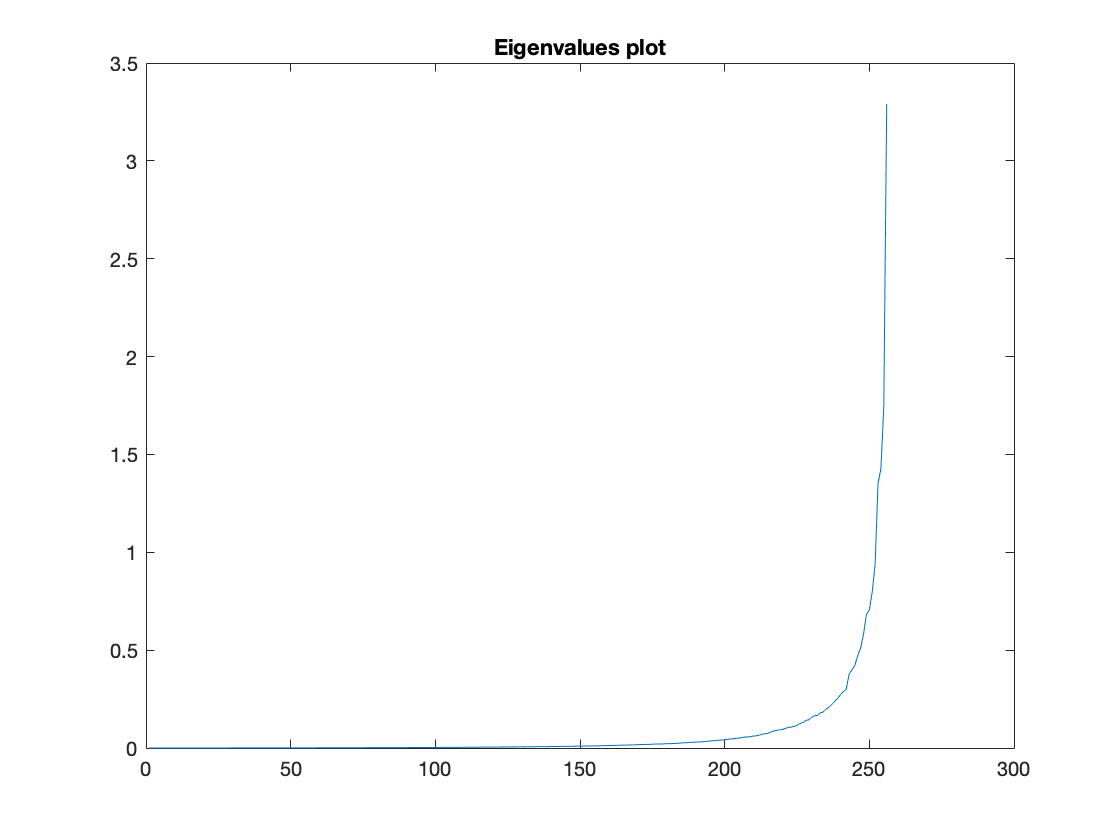
\includegraphics[width=8cm]{images/eigenvalues_plot.png}
    \caption{Eigenvalues plot}
    \label{fig:10}
\end{figure}

\begin{figure}[h]
    \centering
    \begin{subfigure}[b]{0.32\textwidth}
    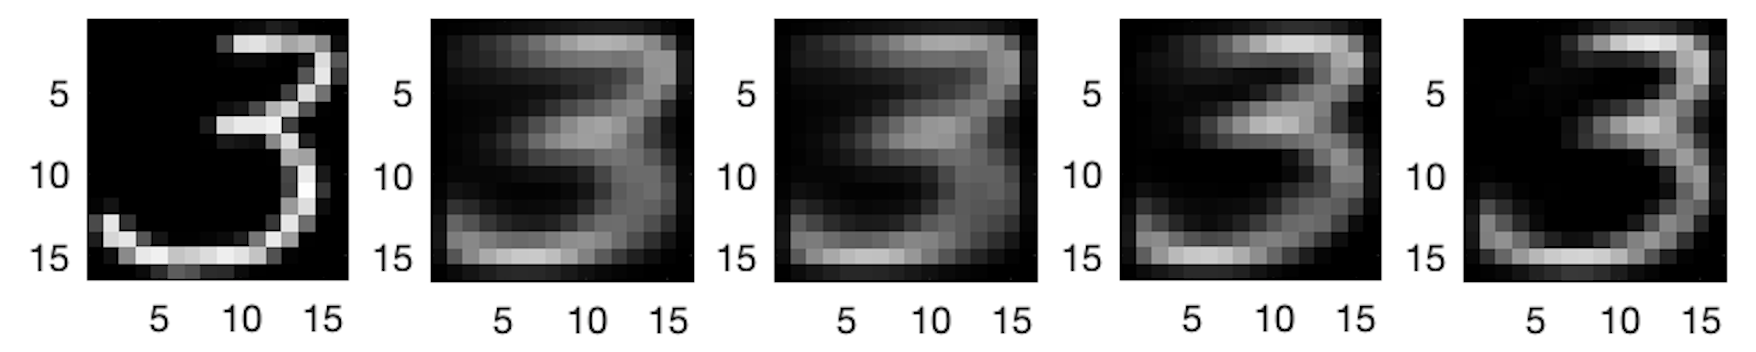
\includegraphics[width=\linewidth]{images/3s.png}
    \caption{Mean}
    \end{subfigure}
    \begin{subfigure}[b]{0.32\textwidth}
    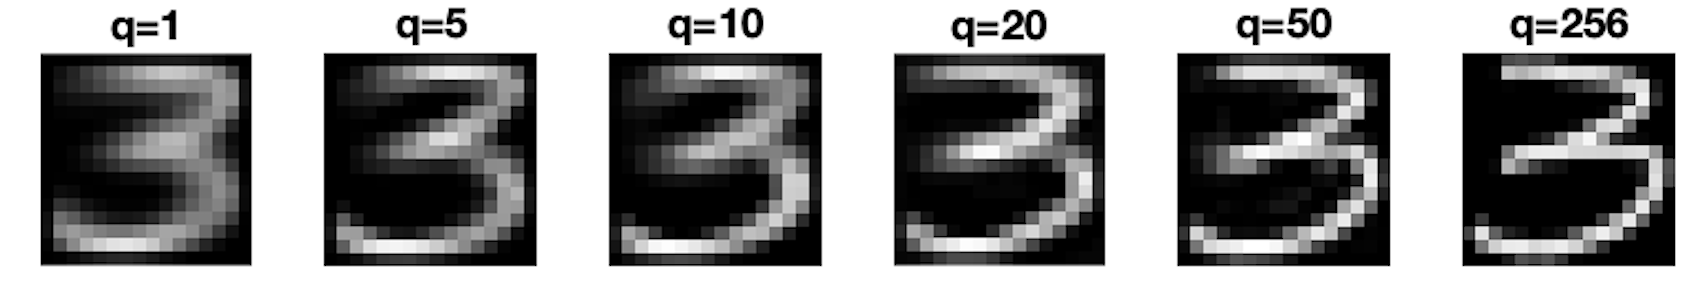
\includegraphics[width=\linewidth]{images/3s_recon.png}
    \caption{Reconstructed}
    \end{subfigure}
    \caption{Threes mean and reconstructed images}
    \label{fig:11}
\end{figure}

\begin{figure}[h]
    \centering
    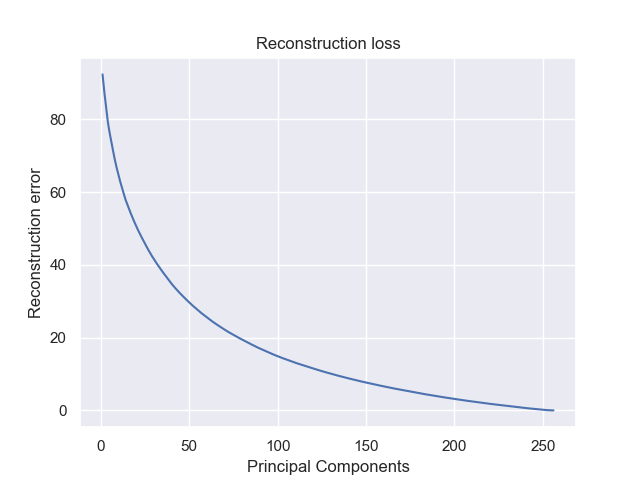
\includegraphics[width=8cm]{images/reconloss.png}
    \caption{Reconstruction loss}
    \label{fig:12}
\end{figure}

\subsection{Stacked Autoencoders}
An autoencoder is a type of neural network that is used to learn encodings of data in an unsupervised manner. Autoencoders have an internal hidden layer that consists of an \textit{encoder}, whose responsibility is to map the input to the code, and a \textit{decoder} that maps it to a reconstruction of the initial input. They are typically used for dimensionality reduction and feature learning. Additionally, apart from their reduction end, there is also a reconstruction side that tries to generate a representation as close as possible to the original input.  

Stacked autoencoders are neural networks that consist by combining multiple layers of sparse autoencoders in which the inputs of each successive layer are wired to the inputs of the preceding layer and are trained in a greedy layer-wise fashion. The objective of this exercise was to train a stacked autoencoder model to classify images that represent handwritten digits. In order to better understand their functionality and to evaluate their performance, we need to investigate the effect that their parameters have. The architecture of the network is comprised by 3 hidden layers and 2 different models were investigated. The first model includes two layers that consist of 40 and 20 hidden neurons and obtains an accuracy score of 0.9663. In the second model we increase the number of neurons for each successive layer to 50 and 100 respectively and we achieve a higher accuracy of 0.9977. Both results are averaged over 10 runs and the number of epochs was 400 for the first layer and 100 for the second one in both cases. Results are shown in Table 2.

The MLP architectures that were deployed to compare with the autoencoders comprised of one hidden layer with 100 neurons and two hidden layers with 100 and 100 neurons and they achieved an accuracy score of 0.9593 and 0.9635 respectively. Compared to the autoencoder models, they perform significantly worse in the same number of runs.
\begin{table}
\begin{subtable}[t]{0.48\textwidth}
\centering
\begin{tabular}[t]{l l l l l l |l l}
\toprule
 Neurons&    &accuracy\\
\midrule
  40 &  &0.9763 &\\
  20  & &\\
\midrule                                                  
\midrule
  50 &  & 0.9977 &\\
  100  & &\\
\midrule
\midrule
  100 &  & 0.9593&\\
\midrule
\midrule
  100 &  & 0.9635\\
  100  & &\\
\bottomrule
\end{tabular}
\end{subtable}
\caption{First two rows: Stacked autoencoders and their accuracy. Second set of rows: MLP and its accuracy.}
\label{tableaut}
\end{table}

\subsection{Convolutional Neural Networks}
Convolutional Neural Networks (CNNs) are a type of deep neural networks that are mostly used to process and analyze images. CNNs are fully connected, multilayer networks and use the concept of local connectivity, in the sense that when we observe datapoints in a dataset that are close to each other it is likely they are more connected than data points that are more distant to each other.

The first part of this exercise is to execute the given script and investigate the CNN's architecture and layers. In particular, the script deploys a pre-trained CNN named AlexNet that aims to classify three different classes of images, namely 'airplanes', 'ferry' and 'laptop'. The first convolutional layer filters the input image of size $227 \times 227 \times 3$ and has 96 kernels of size $11 x 11 x 3$, meaning that the filters in the first convolutional layer have 11 pixels width and height and 3 corresponds to the 3 RGB color channels of the input images. These 96 filters correspond in $96 \times 11 \times 11 x3$ weights, which represent 96 two-dimensional feature maps. The stride is the the filter's pixel shift over the image and it is set to 4 and padding, which represents an extra layer that detects features on the edges of the images, is set to 0. The size of the input image can be calculated by: 
\begin{equation}
 O = \frac{  (I - K + 2P)}{S} + 1
\end{equation}
where $I$ is the input volume, $K$ is the kernel size, $P$ is the padding and $S$ is the stride. In this case, after the first convolutional layer, the output image has size $(227 - 11 /4) + 1 = 55$. Additionally, the first convolutional layer is followed by a max pooling layer, a Rectified Linear Unit (ReLU) layer and a batch normalization layer. The ReLU layer applies the activation function to the input volume of the first layer and the batch normalization layer essentially normalizes the output, therefore they do not affect the dimension of the input volume. The max pooling layer however further reduces the image to $(55 - 3 /2) + 1 = 27$ pixels. 

The second convolutional layer has a stride of 1 and therefore does not further reduce the dimension of the input image. Similarly to the previous convolutional layer, we observe that the second max pooling layer that is applied reduces the input image to $(27 - 3 /2) + 1 = 13$ pixels. The remaining 3 convolutional layers similarly use a stride of 1 and therefore do not affect the dimension of their volume, whereas the final max pooling layer further reduces the dimension of the input volume to $(13 - 3 /2) + 1 = 6$. Finally, in this example, after the fifth convolutional layer we have 3 fully connected layers that consist of 4096, 4096 and 1000 neurons. This means that if we compare the initial input size of $227 \times 227 \times 3 = 154.857$ with the final one that is 1000, we get a significantly smaller vector of neurons.
In the second and final part of this exercise, we deploy a CNN in order to classify handwritten digits derived from the dataset that was used previously. This dataset consists of 10.000 images which are equally divided into 10 different classes representing the handwritten digits from 0 to 9 and we randomly divide the data to training and test set, so that the training set contains 750 images and the test set 250 unseen images, each digit image being of size $28 \times 28 \times 1$. The model architectures investigated in this exercise include a variation of different numbers of convolutional layers (from 1 to 3) and different kernel filters. Every model was tested for 30 epochs with an initial learning rate of 0.0001. Throughout all experiments the activation function is the same (ReLU). All accuracy scores are measured over 10 runs for each model and are presented in Table 3. 

\begin{table}[h]
\centering
\begin{tabular}[t]{l l l l | l}
\toprule
  Model & Architecture & Filters & Kernel &Accuracy\\
\midrule
  1 & conv 1 &   5 x 5 &      2  & 0.5788\\
  &  ReLU &    &       &          \\
  & max pool &   2 x 2 &              \\
  &  FC(10) & \\
  &  softmax & \\
  &  classification & \\
  

\midrule                                                  
  2 & conv 1 &   5 x 5 &      12 &  0.9760\\
  &  ReLU &    &       &          \\
  & max pool &   2 x 2 &       &  \\
  & conv 2 &   5 x 5 &      24 &  \\
  &  ReLU &    &       &          \\
  &  FC(10) & \\
  &  softmax & \\
  &  classification & \\

\midrule                                                  
  3 & conv 1 &   3 x 3 &      12 & 0.9924\\
  &  ReLU &    &       &          \\
  & max pool &   2 x 2 &        \\
  & conv 2 &   3 x 3 &      24 &\\
  &  ReLU &    &       &         \\
  &  FC(10) & \\
  &  softmax & \\
  &  classification & \\
  
\midrule                                                  
  4 & conv 1 &   3 x 3 &      16 & 0.9944\\
  &  ReLU &    &       &          \\
  & max pool &   2 x 2 &        \\
  & conv 2 &   3 x 3 &      32 &\\
  &  ReLU &    &       &          \\
  & conv 3 &   3 x 3 &      48 &\\
  &  FC(10) & \\
  &  softmax & \\
  &  classification & \\

\bottomrule
\end{tabular}

\label{tab:cnn}

\caption{Various architectures used in the experiments and their performance in terms of accuracy.}
\label{cnn}
\end{table}

\section{Generative Models}
\subsection{Restricted Boltzmann Machines}
Restricted Boltzmann Machines (RBM) are generative stochastic neural networks that can learn and represent a probability distribution over their set of inputs. Learning an RBM is achieved by adjusting its parameters so that the probability distribution they provide will fit the training data as much as possible. They have binary-valued hidden and visible units and a matrix of weights that is represents the association between a hidden and a visible unit. Additionally, they consist of bias weights for hidden and visible neurons. Their energy function is similar to Hopfield networks and it defines the probability distributions over neurons. The sets of neurons are arranged in two layers, the first one consisting of the visible units and the second one of the hidden units. They are characterized as restricted due to the way that the visible and hidden units are connected. Specifically, there is no intra-layer communication between hidden and visible units, thus forming a bipartite graph between the two sets of neurons. If this restriction is uplifted, the resulting model is transformed into a Boltzmann machine. 

In this exercise we train an RBM in reconstructing digits from the MNIST handwritten digits database and the aim is to experiment with applying different values to their parameters. These parameters are the number of hidden units, the learning rate and also the number of iterations.Figure 13 illustrates the comparison between the real images and the ones sampled by RBM with 100 hidden units, learning rate 0.03 and number of iterations 30.

\begin{figure}[h]
    \centering
    \begin{subfigure}[b]{0.32\textwidth}
    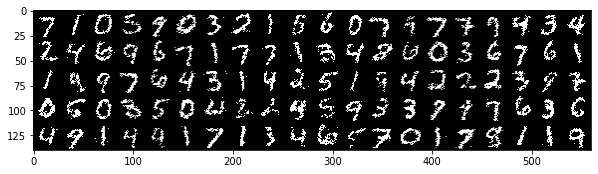
\includegraphics[width=\linewidth]{images/100neurons_30iter.png}
    \caption{Sampled images}
    \end{subfigure}
    \begin{subfigure}[b]{0.32\textwidth}
    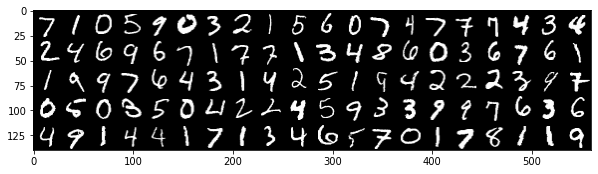
\includegraphics[width=\linewidth]{images/actual_imgs.png}
    \caption{Actual images}
    \end{subfigure}
    \caption{Sampled and real images for the RBM}
    \label{fig:13}
\end{figure}


\textbf{Number of hidden units:} As the number of hidden neurons increases, the performance certainly improves, since the model is able to learn more patterns whereas in contrast, when using a small number of hidden neurons, the network has less flexibility and cannot perform efficient approximations of the data. However, it is important to note that a significantly high number of neurons leads to overfitting because the model tends to memorize the input digits and patterns. It follows that a very small number of neurons may lead to underfitting. 

\textbf{Learning rate:} The learning rate parameter of an RBM controls the update of the weight after each iteration. Very small learning rates decrease the performance since more time is required for the training process whereas very high learning rates result to unstable training. 

\textbf{Iterations:} The number of iterations refers to the number of simulations the model is making during training. It is analogous to the number of epochs and should, in general, not be particularly small so that the model can converge. 

In order to reconstruct unseen images, the number of Gibbs steps has to be increased from 1 which was the case in the previous section. When we increase it to 15, we vary the number of rows to remove from 10 to 15 and 20. The results are shown in Figure 14.

\begin{figure}[h]
    \centering
    \begin{subfigure}[b]{0.32\textwidth}
    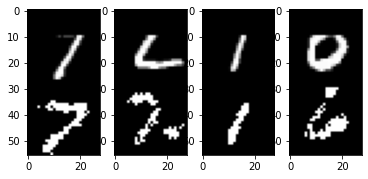
\includegraphics[width=\linewidth]{images/gibbs=15_remove=10.png}
    \caption{Removing 10 rows}
    \end{subfigure}
    \begin{subfigure}[b]{0.32\textwidth}
    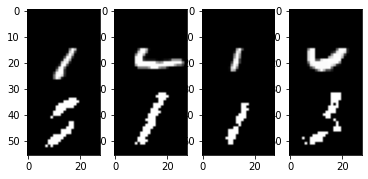
\includegraphics[width=\linewidth]{images/gibbs=15_remove=15.png}
    \caption{Removing 15 rows}
    \end{subfigure}
    \begin{subfigure}[b]{0.32\textwidth}
    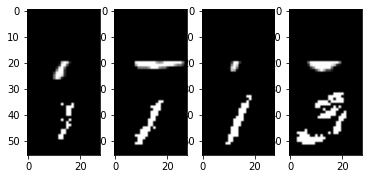
\includegraphics[width=\linewidth]{images/gibbs=15_remove=20.png}
    \caption{Removing 20 rows}
    \end{subfigure}
    \caption{Reconstructing unseen images with Gibbs step 15}
    \label{fig:14}
\end{figure}


\subsection{Deep Boltzmann Machines}
Deep Boltzmann Machines (DBM) are a special case of RBMs with the difference being that they are comprised of more hidden layers which are stacked one onto another. In a DBM with 2 layers, the output of the first hidden layer is used as the input of the second hidden layer, thus the deeper layers can extract more definitive features. Figure 15 illustrates the comparison between components extracted by an RBM and a DBM with 2 layers. 

\begin{figure*}[]
        \centering
        \begin{subfigure}{0.30\linewidth}
            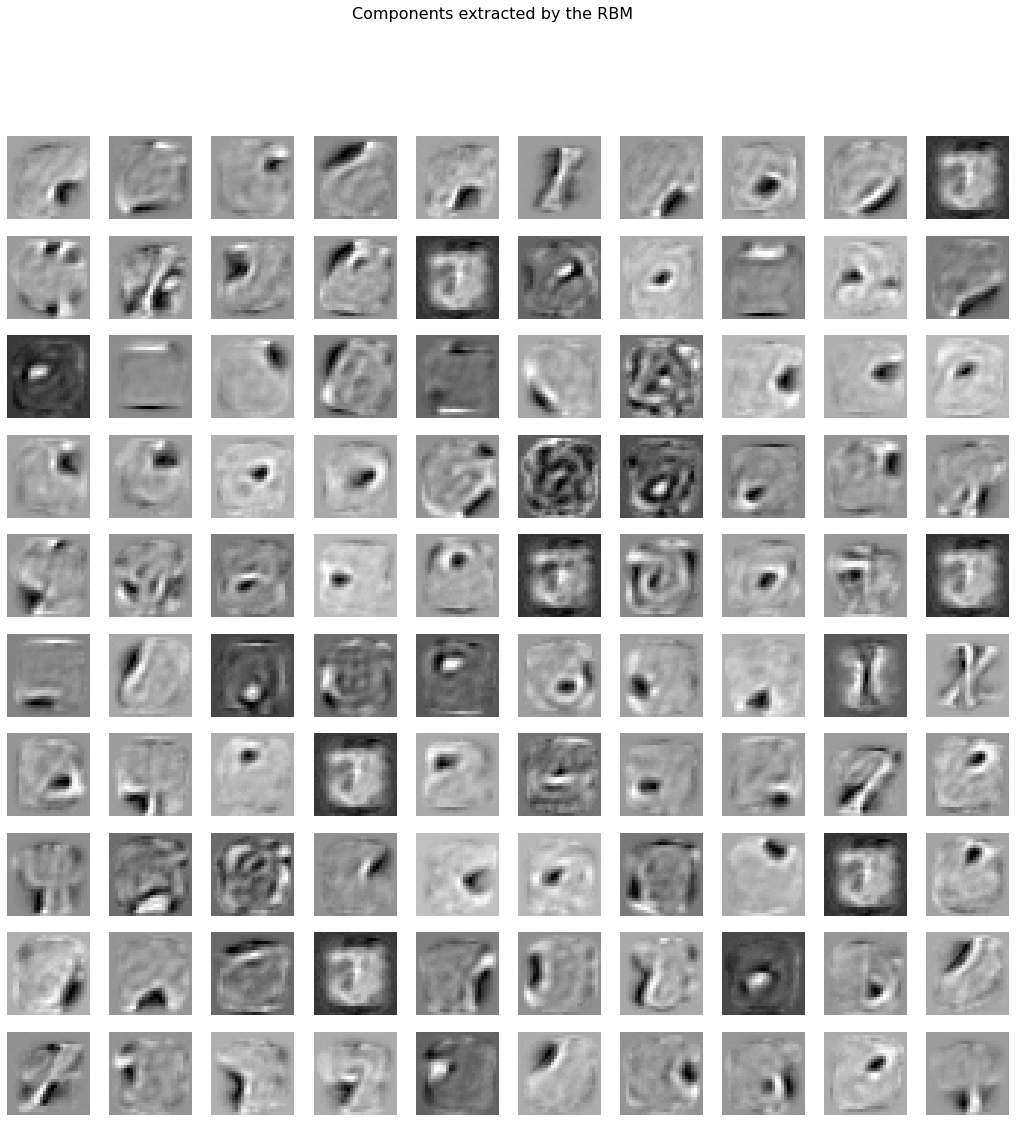
\includegraphics[width=\linewidth]{images/componentsRBM_neur=100.png}
            \caption{RBM}
        \end{subfigure}
         \begin{subfigure}{0.30\linewidth}
            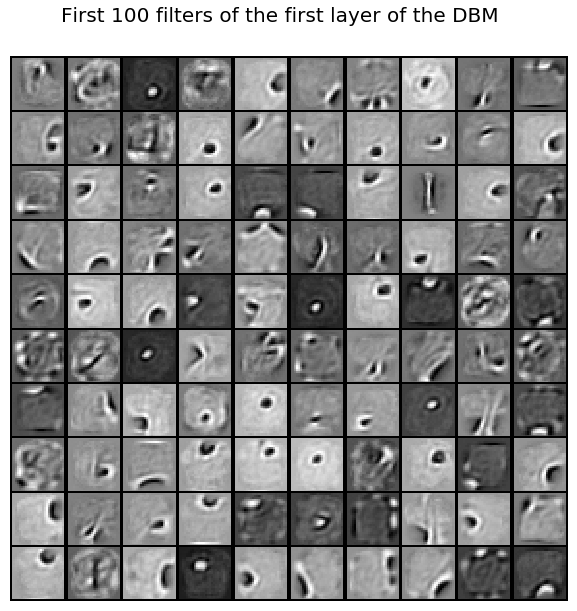
\includegraphics[width=\linewidth]{images/dbm_1.png}
            \caption{First layer}
        \end{subfigure}  
        \begin{subfigure}{0.30\linewidth}
            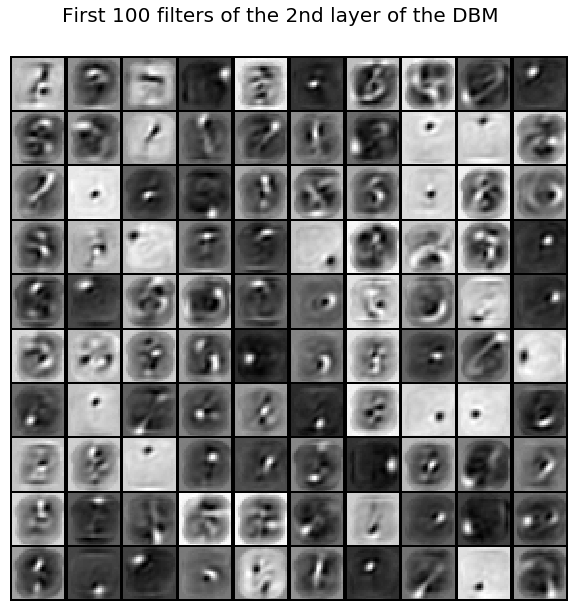
\includegraphics[width=\linewidth]{images/dbm_2.png}
            \caption{Second layer}
        \end{subfigure}        
        \caption{ Visualization of (a) the components extracted by RBM (b) The filters in the first layer (c) and in the Second layer of a DBM }
        \label{fig:15}
\end{figure*}

\subsection{Generative Adversarial Networks}
Generative Adversarial Networks (GANs) are algorithmic structures that use two neural networks that compete against each other in order to synthesize new instances of data that resemble real data. One neural network, the \textit{generator}, is responsible for creating new instances of data while the other, the \textit{discriminator}, evaluates them for authenticity, deciding whether the generated new data instance belongs to the actual training dataset or not. The generator takes as input a vector of random numbers and outputs it as an image which is fed to the discriminator. The discriminator is fed with both real and fake images and returns a prediction in terms of probability, where 1 means the image is real and 0 means the image is fake. 

The objective of this exercise is to train a deep convolutional adversarial network (DCGAN) in the CIFAR-10 dataset, which consists of 60000 32x32 colour images in 10 classes, with 6000 images per class. The class chosen for this experiment was number 3 which refers to cat images. After training the DCGAN for different number of batches and different batch size, we obtain the result that is depicted in Figure 16. The results are certainly improved when training with a higher number of batches but the images created remain somewhat blurry. At the beginning of the training the discriminator demonstrates much higher accuracy and lower loss than the generator. During the training these percentages eventually even out since both models improve in a parallel manner. 
 
\subsection{Optimal Transport}
In the color transfer problem the objective is to transfer the color palette of an image into another, turning the second image visually similar to the first one, in terms of their color. If we consider these colors as distribution, we can apply Optimal Transport (OT), a popular mathematical framework for minimizing the distance between two probability distributions. The aim of this exercise is to experiment with two different optimal transport algorithmic models, each one using its own distance metric. The first one uses the Wasserstein metric and the second one the Sinkhorn distance. The main advantage of Sinkhorn distance is that it regularizes the the distance between the two color distributions by applying entropy constraints that render the distribution into more homogeneous, providing therefore a more smooth representation that the Wasserstein distance. The results of applying the two different algorithms are shown in Figure 17.

\begin{figure*}[]
    \centering
    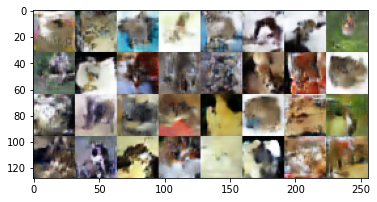
\includegraphics[width=0.8\linewidth]{images/dcgan_cats_30k_128.png}
    \caption{Images of cats produced by the DCGAN}
    \label{fig:16}
\end{figure*}

\begin{figure*}[]
    \centering
    \begin{subfigure}{0.50\linewidth}
        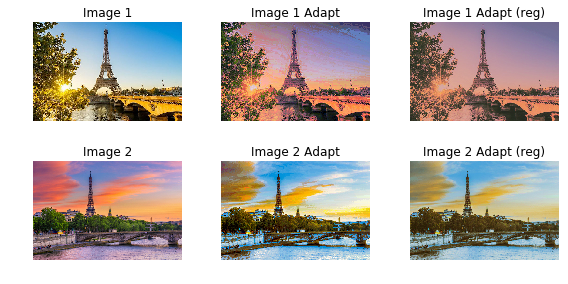
\includegraphics[width=\linewidth]{images/ot.png}
    \end{subfigure}	        
    \caption{Color transfer with Wasserstein and Sinkhorn  OT algorithms}
    \label{fig:17}
\end{figure*}

\subsection{Fully Connected MiniMax GAN and Wasserstein GAN}
In this exercise the objective is to train a minimax GAN and a Wasserstein GAN (WGAN) in the MNIST dataset and then compare their performances. WGANs implement a new loss function that essentially transforms the discriminator from a classifier to a critic that scores the realness or fakeness of images. This loss function is the Wasserstein distance, which was explained in the previous section. Minimax GAN models generally suffer from the problem of weight clipping, which happens when weights get trapped between two min and max value. This is addressed by WGANs by introducing a gradient penalty or weight penalty which restricts some gradients from explodingor vanishing, meaning it restricts them from getting min or max values and get trapped between those two. Another significant advantage of WGANs over standard GANs is that they do not suffer from mode collapse, which occurs in standard GANs when the generator does not produce enough diverse samples and therefore the discriminator will only discriminate between a small set of samples. Overall, for the reasons mentioned above, WGANs are considered to be more stable than standard GANs and produce results of higher quality. Figure 18 illustrates the difference between the outputs of a standard GAN and a WGAN. 

\begin{figure*}[]
        \centering
         \begin{subfigure}{0.40\linewidth}
            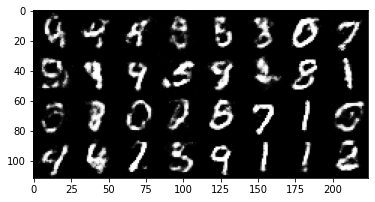
\includegraphics[width=\linewidth]{images/wgan_rep.png}
            \caption{WGAN}
        \end{subfigure}  
        \begin{subfigure}{0.40\linewidth}
            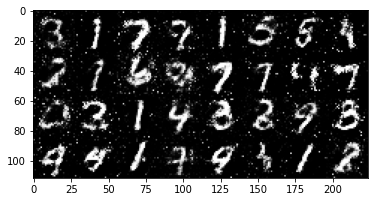
\includegraphics[width=\linewidth]{images/gan_rep.png}
            \caption{standard GAN}
        \end{subfigure}
		        
        \caption{Performance comparison of a WGAN and a standard minimax GAN}
        \label{fig:18}
\end{figure*}

\ifCLASSOPTIONcompsoc

\end{document}


